\documentclass[twoside]{book}

% Packages required by doxygen
\usepackage{fixltx2e}
\usepackage{calc}
\usepackage{doxygen}
\usepackage[export]{adjustbox} % also loads graphicx
\usepackage{graphicx}
\usepackage[utf8]{inputenc}
\usepackage{makeidx}
\usepackage{multicol}
\usepackage{multirow}
\PassOptionsToPackage{warn}{textcomp}
\usepackage{textcomp}
\usepackage[nointegrals]{wasysym}
\usepackage[table]{xcolor}

% Font selection
\usepackage[T1]{fontenc}
\usepackage[scaled=.90]{helvet}
\usepackage{courier}
\usepackage{amssymb}
\usepackage{sectsty}
\renewcommand{\familydefault}{\sfdefault}
\allsectionsfont{%
  \fontseries{bc}\selectfont%
  \color{darkgray}%
}
\renewcommand{\DoxyLabelFont}{%
  \fontseries{bc}\selectfont%
  \color{darkgray}%
}
\newcommand{\+}{\discretionary{\mbox{\scriptsize$\hookleftarrow$}}{}{}}

% Page & text layout
\usepackage{geometry}
\geometry{%
  a4paper,%
  top=2.5cm,%
  bottom=2.5cm,%
  left=2.5cm,%
  right=2.5cm%
}
\tolerance=750
\hfuzz=15pt
\hbadness=750
\setlength{\emergencystretch}{15pt}
\setlength{\parindent}{0cm}
\setlength{\parskip}{3ex plus 2ex minus 2ex}
\makeatletter
\renewcommand{\paragraph}{%
  \@startsection{paragraph}{4}{0ex}{-1.0ex}{1.0ex}{%
    \normalfont\normalsize\bfseries\SS@parafont%
  }%
}
\renewcommand{\subparagraph}{%
  \@startsection{subparagraph}{5}{0ex}{-1.0ex}{1.0ex}{%
    \normalfont\normalsize\bfseries\SS@subparafont%
  }%
}
\makeatother

% Headers & footers
\usepackage{fancyhdr}
\pagestyle{fancyplain}
\fancyhead[LE]{\fancyplain{}{\bfseries\thepage}}
\fancyhead[CE]{\fancyplain{}{}}
\fancyhead[RE]{\fancyplain{}{\bfseries\leftmark}}
\fancyhead[LO]{\fancyplain{}{\bfseries\rightmark}}
\fancyhead[CO]{\fancyplain{}{}}
\fancyhead[RO]{\fancyplain{}{\bfseries\thepage}}
\fancyfoot[LE]{\fancyplain{}{}}
\fancyfoot[CE]{\fancyplain{}{}}
\fancyfoot[RE]{\fancyplain{}{\bfseries\scriptsize Generated by Doxygen }}
\fancyfoot[LO]{\fancyplain{}{\bfseries\scriptsize Generated by Doxygen }}
\fancyfoot[CO]{\fancyplain{}{}}
\fancyfoot[RO]{\fancyplain{}{}}
\renewcommand{\footrulewidth}{0.4pt}
\renewcommand{\chaptermark}[1]{%
  \markboth{#1}{}%
}
\renewcommand{\sectionmark}[1]{%
  \markright{\thesection\ #1}%
}

% Indices & bibliography
\usepackage{natbib}
\usepackage[titles]{tocloft}
\setcounter{tocdepth}{3}
\setcounter{secnumdepth}{5}
\makeindex

% Hyperlinks (required, but should be loaded last)
\usepackage{ifpdf}
\ifpdf
  \usepackage[pdftex,pagebackref=true]{hyperref}
\else
  \usepackage[ps2pdf,pagebackref=true]{hyperref}
\fi
\hypersetup{%
  colorlinks=true,%
  linkcolor=blue,%
  citecolor=blue,%
  unicode%
}

% Custom commands
\newcommand{\clearemptydoublepage}{%
  \newpage{\pagestyle{empty}\cleardoublepage}%
}

\usepackage{caption}
\captionsetup{labelsep=space,justification=centering,font={bf},singlelinecheck=off,skip=4pt,position=top}

%===== C O N T E N T S =====

\begin{document}

% Titlepage & ToC
\hypersetup{pageanchor=false,
             bookmarksnumbered=true,
             pdfencoding=unicode
            }
\pagenumbering{roman}
\begin{titlepage}
\vspace*{7cm}
\begin{center}%
{\Large F\+D\+CL Controllers }\\
\vspace*{1cm}
{\large Generated by Doxygen 1.8.11}\\
\end{center}
\end{titlepage}
\clearemptydoublepage
\tableofcontents
\clearemptydoublepage
\pagenumbering{arabic}
\hypersetup{pageanchor=true}

%--- Begin generated contents ---
\chapter{F\+D\+CL Controllers in C++}
\label{index}\hypertarget{index}{}\subsection*{Compiling}

Following instructions assume you have git already installed in your system.


\begin{DoxyEnumerate}
\item Install dependencies. 
\begin{DoxyCode}
1 # Linux
2 sudo apt-get install -y cmake pkg-config
3 
4 # Mac
5 brew install cmake pkg-config
\end{DoxyCode}

\item Update submodules 
\begin{DoxyCode}
1 git submodule update --init --recursive
\end{DoxyCode}

\item Setup compile directory inside the {\ttfamily cpp} directory. 
\begin{DoxyCode}
1 mkdir build
2 cd build
3 cmake ../
\end{DoxyCode}

\item Compile and run. 
\begin{DoxyCode}
1 make example
2 ./example
\end{DoxyCode}

\end{DoxyEnumerate}

For more information, make sure to check the {\ttfamily Classes} tab.

\subsection*{Unit Tests}


\begin{DoxyEnumerate}
\item Build the unit tests first\+: 
\begin{DoxyCode}
1 make test\_all
\end{DoxyCode}

\item Run the unit test 
\begin{DoxyCode}
1 ./test\_all
\end{DoxyCode}
 All the tests must pass.
\end{DoxyEnumerate}

\subsection*{Generating the Documentation}

This C++ code is documented using Doxygen. Doxygen automatically generates the documentation based on the comments in header files.

If you want to update the documentation, follow the below steps.
\begin{DoxyEnumerate}
\item If not already installed, install {\ttfamily doxygen}\+: 
\begin{DoxyCode}
1 # Linux
2 sudo apt-get install -y doxygen graphviz
3 
4 # Mac
5 brew install graphviz doxygen
\end{DoxyCode}

\end{DoxyEnumerate}
\begin{DoxyEnumerate}
\item Run doxygen (from {\ttfamily master} branch) 
\begin{DoxyCode}
1 cd Doxygen
2 doxygen Doxyfile
\end{DoxyCode}
 
\end{DoxyEnumerate}
\chapter{Class Index}
\section{Class List}
Here are the classes, structs, unions and interfaces with brief descriptions\+:\begin{DoxyCompactList}
\item\contentsline{section}{\hyperlink{classfdcl_1_1command__t}{fdcl\+::command\+\_\+t} \\*Data structure to store command (or desired) values }{\pageref{classfdcl_1_1command__t}}{}
\item\contentsline{section}{\hyperlink{classfdcl_1_1control}{fdcl\+::control} \\*Controller functions for the rover }{\pageref{classfdcl_1_1control}}{}
\item\contentsline{section}{\hyperlink{structfdcl_1_1integral__error}{fdcl\+::integral\+\_\+error} \\*Integral for error for a double }{\pageref{structfdcl_1_1integral__error}}{}
\item\contentsline{section}{\hyperlink{structfdcl_1_1integral__error__vec3}{fdcl\+::integral\+\_\+error\+\_\+vec3} \\*Integral for error for Vector3 }{\pageref{structfdcl_1_1integral__error__vec3}}{}
\item\contentsline{section}{\hyperlink{classfdcl_1_1param}{fdcl\+::param} \\*Saving and loading parameters }{\pageref{classfdcl_1_1param}}{}
\item\contentsline{section}{\hyperlink{structfdcl_1_1state__t}{fdcl\+::state\+\_\+t} \\*Data structure to store current states }{\pageref{structfdcl_1_1state__t}}{}
\end{DoxyCompactList}

\chapter{File Index}
\section{File List}
Here is a list of all documented files with brief descriptions\+:\begin{DoxyCompactList}
\item\contentsline{section}{cpp/include/\hyperlink{common__types_8hpp}{common\+\_\+types.\+hpp} \\*Data types used throughout the code }{\pageref{common__types_8hpp}}{}
\item\contentsline{section}{cpp/include/fdcl/\hyperlink{control_8hpp}{control.\+hpp} \\*Control class used to generate motors outputs for a desired trajectory }{\pageref{control_8hpp}}{}
\item\contentsline{section}{cpp/include/fdcl/\hyperlink{integral__utils_8hpp}{integral\+\_\+utils.\+hpp} \\*Structures to handle integral errors }{\pageref{integral__utils_8hpp}}{}
\item\contentsline{section}{cpp/include/fdcl/\hyperlink{matrix__utils_8hpp}{matrix\+\_\+utils.\+hpp} \\*Miscellaneous math functions }{\pageref{matrix__utils_8hpp}}{}
\item\contentsline{section}{cpp/libraries/fdcl\+\_\+param/include/fdcl/{\bfseries param.\+hpp} }{\pageref{param_8hpp}}{}
\end{DoxyCompactList}

\chapter{Class Documentation}
\hypertarget{classfdcl_1_1command__t}{}\section{fdcl\+:\+:command\+\_\+t Class Reference}
\label{classfdcl_1_1command__t}\index{fdcl\+::command\+\_\+t@{fdcl\+::command\+\_\+t}}


Data structure to store command (or desired) values.  




{\ttfamily \#include $<$include/common\+\_\+types.\+hpp$>$}

\subsection*{Public Attributes}
\begin{DoxyCompactItemize}
\item 
Vector3 {\bfseries Wd} = Vector3\+::\+Zero()\hypertarget{classfdcl_1_1command__t_a951c228eb6c8cabcdd3fffd3d378fd0a}{}\label{classfdcl_1_1command__t_a951c228eb6c8cabcdd3fffd3d378fd0a}

\item 
Vector3 {\bfseries Wd\+\_\+dot} = Vector3\+::\+Zero()\hypertarget{classfdcl_1_1command__t_a089d1bf0a2be6eecd25f1dc0b3b218e2}{}\label{classfdcl_1_1command__t_a089d1bf0a2be6eecd25f1dc0b3b218e2}

\item 
Vector3 {\bfseries Wd\+\_\+2dot} = Vector3\+::\+Zero()\hypertarget{classfdcl_1_1command__t_a11e06c9ee098901b9a4705a5f9b88902}{}\label{classfdcl_1_1command__t_a11e06c9ee098901b9a4705a5f9b88902}

\item 
Matrix3 {\bfseries Rd} = Matrix3\+::\+Identity()\hypertarget{classfdcl_1_1command__t_a95208aed71ff193f8d98813b52fc4920}{}\label{classfdcl_1_1command__t_a95208aed71ff193f8d98813b52fc4920}

\item 
Vector3 {\bfseries xd} = Vector3\+::\+Zero()\hypertarget{classfdcl_1_1command__t_a5540e79f1b8c99c8853c568d02ea2e34}{}\label{classfdcl_1_1command__t_a5540e79f1b8c99c8853c568d02ea2e34}

\item 
Vector3 {\bfseries xd\+\_\+dot} = Vector3\+::\+Zero()\hypertarget{classfdcl_1_1command__t_a02aa804c1d8e34f58ae030d9619dcda5}{}\label{classfdcl_1_1command__t_a02aa804c1d8e34f58ae030d9619dcda5}

\item 
Vector3 {\bfseries xd\+\_\+2dot} = Vector3\+::\+Zero()\hypertarget{classfdcl_1_1command__t_a01a7b45dc7c4e7b82e0916791d4ea3ef}{}\label{classfdcl_1_1command__t_a01a7b45dc7c4e7b82e0916791d4ea3ef}

\item 
Vector3 {\bfseries xd\+\_\+3dot} = Vector3\+::\+Zero()\hypertarget{classfdcl_1_1command__t_af96028068e13bc9697b70e661d6d315a}{}\label{classfdcl_1_1command__t_af96028068e13bc9697b70e661d6d315a}

\item 
Vector3 {\bfseries xd\+\_\+4dot} = Vector3\+::\+Zero()\hypertarget{classfdcl_1_1command__t_ae647f943a3674680f01e2d05e1255efe}{}\label{classfdcl_1_1command__t_ae647f943a3674680f01e2d05e1255efe}

\item 
Vector3 {\bfseries b1d} = Vector3\+::\+Zero()\hypertarget{classfdcl_1_1command__t_a8f718c955249a599cfbccd313c2159a7}{}\label{classfdcl_1_1command__t_a8f718c955249a599cfbccd313c2159a7}

\item 
Vector3 {\bfseries b1d\+\_\+dot} = Vector3\+::\+Zero()\hypertarget{classfdcl_1_1command__t_a98db88614732d13719aa486c08731fac}{}\label{classfdcl_1_1command__t_a98db88614732d13719aa486c08731fac}

\item 
Vector3 {\bfseries b1d\+\_\+ddot} = Vector3\+::\+Zero()\hypertarget{classfdcl_1_1command__t_ad3ce53fd2ec89431d2142673ed4fe405}{}\label{classfdcl_1_1command__t_ad3ce53fd2ec89431d2142673ed4fe405}

\item 
Vector3 {\bfseries b3d} = Vector3\+::\+Zero()\hypertarget{classfdcl_1_1command__t_a945a0af72751d12dfb3212715d23f376}{}\label{classfdcl_1_1command__t_a945a0af72751d12dfb3212715d23f376}

\item 
Vector3 {\bfseries b3d\+\_\+dot} = Vector3\+::\+Zero()\hypertarget{classfdcl_1_1command__t_a6af701193b4342962e44685670693ed7}{}\label{classfdcl_1_1command__t_a6af701193b4342962e44685670693ed7}

\item 
Vector3 {\bfseries b3d\+\_\+ddot} = Vector3\+::\+Zero()\hypertarget{classfdcl_1_1command__t_a13f676f181ece67172103bf8b620bd5c}{}\label{classfdcl_1_1command__t_a13f676f181ece67172103bf8b620bd5c}

\item 
Vector3 {\bfseries b1c} = Vector3\+::\+Zero()\hypertarget{classfdcl_1_1command__t_af120c4e294663ebb78dbc6d621dd975d}{}\label{classfdcl_1_1command__t_af120c4e294663ebb78dbc6d621dd975d}

\item 
double {\bfseries wc3} = 0.\+0\hypertarget{classfdcl_1_1command__t_a19d3b46a52378548cb0670c32ff27269}{}\label{classfdcl_1_1command__t_a19d3b46a52378548cb0670c32ff27269}

\item 
double {\bfseries wc3\+\_\+dot} = 0.\+0\hypertarget{classfdcl_1_1command__t_a59b308f32e194eeae8d6a0dc9a9ccb80}{}\label{classfdcl_1_1command__t_a59b308f32e194eeae8d6a0dc9a9ccb80}

\item 
Vector3 {\bfseries b1} = Vector3\+::\+Zero()\hypertarget{classfdcl_1_1command__t_ad7df0cf47e259dd108444e987a882135}{}\label{classfdcl_1_1command__t_ad7df0cf47e259dd108444e987a882135}

\item 
Vector3 {\bfseries b2} = Vector3\+::\+Zero()\hypertarget{classfdcl_1_1command__t_a36f9672461220c509e01f8346ed422c2}{}\label{classfdcl_1_1command__t_a36f9672461220c509e01f8346ed422c2}

\item 
Vector3 {\bfseries b3} = Vector3\+::\+Zero()\hypertarget{classfdcl_1_1command__t_a9c4eccec9e1b04d87dab61e0f56d78c2}{}\label{classfdcl_1_1command__t_a9c4eccec9e1b04d87dab61e0f56d78c2}

\end{DoxyCompactItemize}


\subsection{Detailed Description}
Data structure to store command (or desired) values. 

The documentation for this class was generated from the following file\+:\begin{DoxyCompactItemize}
\item 
cpp/include/\hyperlink{common__types_8hpp}{common\+\_\+types.\+hpp}\end{DoxyCompactItemize}

\hypertarget{classfdcl_1_1control}{}\section{fdcl\+:\+:control Class Reference}
\label{classfdcl_1_1control}\index{fdcl\+::control@{fdcl\+::control}}


Controller functions for the rover.  




{\ttfamily \#include $<$include/fdcl/control.\+hpp$>$}



Collaboration diagram for fdcl\+:\+:control\+:\nopagebreak
\begin{figure}[H]
\begin{center}
\leavevmode
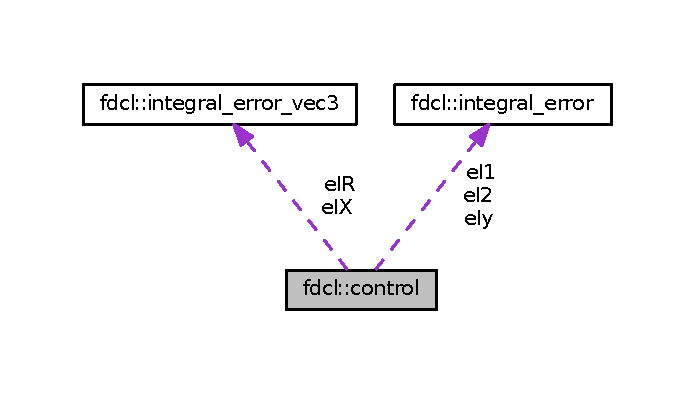
\includegraphics[width=334pt]{classfdcl_1_1control__coll__graph}
\end{center}
\end{figure}
\subsection*{Public Member Functions}
\begin{DoxyCompactItemize}
\item 
\hyperlink{classfdcl_1_1control_ab3bd5c178f3fd6d61bf0f29ad2fc339a}{control} (\hyperlink{structfdcl_1_1state__t}{fdcl\+::state\+\_\+t} $\ast$\&state\+\_\+, \hyperlink{classfdcl_1_1command__t}{fdcl\+::command\+\_\+t} $\ast$\&command\+\_\+, \hyperlink{classfdcl_1_1param}{fdcl\+::param} $\ast$config\+\_\+file\+\_\+)
\item 
void \hyperlink{classfdcl_1_1control_af34df47cf02b52fec6dfc2a4c7e5d371}{init} (void)
\item 
void \hyperlink{classfdcl_1_1control_ad3018fbc5248444a600eabe7f9e8da7d}{load\+\_\+config} (void)
\item 
void \hyperlink{classfdcl_1_1control_af1ddb6b0713fbef94fe71b48e03537bf}{set\+\_\+error\+\_\+to\+\_\+zero} (void)
\item 
void \hyperlink{classfdcl_1_1control_ad4ff4c4944a54ddd2300978cc24c0b3e}{attitude\+\_\+control} (void)
\item 
void \hyperlink{classfdcl_1_1control_a4f2e692c9094316f378a31e8eda35dd0}{attitude\+\_\+control\+\_\+decoupled\+\_\+yaw} (void)
\item 
void \hyperlink{classfdcl_1_1control_a7d2920ae66a3939cdf60ff433e4312b6}{position\+\_\+control} (void)
\item 
double \hyperlink{classfdcl_1_1control_ab88fc7a360808e8c7ee506b78f66ca4a}{get\+\_\+time} (void)
\item 
void \hyperlink{classfdcl_1_1control_a1adfef77a80a920babeaf9dd3ac53a0f}{output\+\_\+uav\+\_\+properties} (double \&m, Matrix3 \&J)
\item 
void \hyperlink{classfdcl_1_1control_a132aa3639cff3b5e2e20da91698216aa}{output\+\_\+fM} (double \&f, Vector3 \&\hyperlink{classfdcl_1_1control_afdd2524a3a5bb05b7235fdca829be124}{M})
\end{DoxyCompactItemize}
\subsection*{Public Attributes}
\begin{DoxyCompactItemize}
\item 
double \hyperlink{classfdcl_1_1control_a85f288d9d87aeb6d6d5509235c4648d9}{t} = 0.\+0
\item 
double \hyperlink{classfdcl_1_1control_ae8000fb9172118f05c69f9fb265b55ef}{t\+\_\+pre} = 0.\+0
\item 
double \hyperlink{classfdcl_1_1control_ab88203b25382616db08db2f4a3cea481}{dt} = 1e-\/9
\item 
int \hyperlink{classfdcl_1_1control_addf63b932fa19bddee426be333843fcb}{freq} = 100
\item 
bool \hyperlink{classfdcl_1_1control_a02b30bdec43753deab3f657562a59065}{use\+\_\+integral} = false
\item 
\hyperlink{structfdcl_1_1integral__error__vec3}{fdcl\+::integral\+\_\+error\+\_\+vec3} \hyperlink{classfdcl_1_1control_ab59f7fd938d291ec387a820eb766a2a5}{e\+IR}
\item 
\hyperlink{structfdcl_1_1integral__error}{fdcl\+::integral\+\_\+error} \hyperlink{classfdcl_1_1control_aa8cc0bd5f3521e4c0460f086b0d81166}{e\+I1}
\item 
\hyperlink{structfdcl_1_1integral__error}{fdcl\+::integral\+\_\+error} \hyperlink{classfdcl_1_1control_aaae1fb8260741f98f50009d4205b940e}{e\+I2}
\item 
\hyperlink{structfdcl_1_1integral__error}{fdcl\+::integral\+\_\+error} \hyperlink{classfdcl_1_1control_a1d33b4d53f99c73983fdbe70ce506ce8}{e\+Iy}
\item 
\hyperlink{structfdcl_1_1integral__error__vec3}{fdcl\+::integral\+\_\+error\+\_\+vec3} \hyperlink{classfdcl_1_1control_a2d7453277a587c8c9b556505f3e3958c}{e\+IX}
\item 
Vector3 \hyperlink{classfdcl_1_1control_af3d563b76ffba90a299349b0968d2b1e}{eR} = Vector3\+::\+Zero()
\item 
Vector3 \hyperlink{classfdcl_1_1control_a3831084838463bafbf25ad50ce39df6d}{eW} = Vector3\+::\+Zero()
\item 
Vector3 \hyperlink{classfdcl_1_1control_a4a67e30ea06e07869210033406cf58cb}{ei} = Vector3\+::\+Zero()
\item 
Vector3 \hyperlink{classfdcl_1_1control_afdd2524a3a5bb05b7235fdca829be124}{M} = Vector3\+::\+Zero()
\item 
Vector3 \hyperlink{classfdcl_1_1control_ad32044f0b435db25f67e5c2f4a5d91d8}{eX} = Vector3\+::\+Zero()
\item 
Vector3 \hyperlink{classfdcl_1_1control_aa0c21496bf7ffffa421e6431c1581bad}{eV} = Vector3\+::\+Zero()
\item 
Vector3 \hyperlink{classfdcl_1_1control_a5ba3e080f42c5ffb282b948b44f3b877}{b1} = Vector3\+::\+Zero()
\item 
Vector3 \hyperlink{classfdcl_1_1control_a6d578fe584100b8f07e9dc6ff7ca01e0}{b2} = Vector3\+::\+Zero()
\item 
Vector3 \hyperlink{classfdcl_1_1control_a7f1776cc82d2375ff788a639baa4064b}{b3} = Vector3\+::\+Zero()
\item 
Vector3 \hyperlink{classfdcl_1_1control_a6c9ba83faa7eae7dde44e9619e08d726}{b3\+\_\+dot} = Vector3\+::\+Zero()
\item 
Eigen\+::\+Matrix$<$ double, 4, 4 $>$ \hyperlink{classfdcl_1_1control_ae111bb213798d710e4ce5b0392a8ab18}{f\+M\+\_\+to\+\_\+forces\+\_\+inv}
\item 
Vector4 \hyperlink{classfdcl_1_1control_aaad0595254a9a993566163d813830491}{f\+\_\+motor}
\item 
Vector4 \hyperlink{classfdcl_1_1control_ac27cf9d04a9f9157eb275eaac60c066d}{fM} = Vector4\+::\+Zero()
\item 
double \hyperlink{classfdcl_1_1control_a14297e7595c3f41cd953a34c767c24f0}{f\+\_\+total} = 0.\+0
\end{DoxyCompactItemize}


\subsection{Detailed Description}
Controller functions for the rover. 

This class includes all the controllers used to control the rover All controller related functions for the rover are included in this class. This inlcudes two attitude controllers, a geometric controller and a decoupled-\/yaw controller (A\+C\+C-\/2019) with a geometric position controller. 

\subsection{Constructor \& Destructor Documentation}
\index{fdcl\+::control@{fdcl\+::control}!control@{control}}
\index{control@{control}!fdcl\+::control@{fdcl\+::control}}
\subsubsection[{\texorpdfstring{control(fdcl\+::state\+\_\+t $\ast$\&state\+\_\+, fdcl\+::command\+\_\+t $\ast$\&command\+\_\+, fdcl\+::param $\ast$config\+\_\+file\+\_\+)}{control(fdcl::state_t *&state_, fdcl::command_t *&command_, fdcl::param *config_file_)}}]{\setlength{\rightskip}{0pt plus 5cm}fdcl\+::control\+::control (
\begin{DoxyParamCaption}
\item[{{\bf fdcl\+::state\+\_\+t} $\ast$\&}]{state\+\_\+, }
\item[{{\bf fdcl\+::command\+\_\+t} $\ast$\&}]{command\+\_\+, }
\item[{{\bf fdcl\+::param} $\ast$}]{config\+\_\+file\+\_\+}
\end{DoxyParamCaption}
)}\hypertarget{classfdcl_1_1control_ab3bd5c178f3fd6d61bf0f29ad2fc339a}{}\label{classfdcl_1_1control_ab3bd5c178f3fd6d61bf0f29ad2fc339a}

\begin{DoxyParams}{Parameters}
{\em state\+\_\+} & Pointer to the current states \\
\hline
{\em command\+\_\+} & Pointer to the desired states \\
\hline
{\em config\+\_\+file\+\_\+} & Pointer to the external \hyperlink{classfdcl_1_1param}{fdcl\+::param} object, which is used to load configuration parameters \\
\hline
\end{DoxyParams}


\subsection{Member Function Documentation}
\index{fdcl\+::control@{fdcl\+::control}!attitude\+\_\+control@{attitude\+\_\+control}}
\index{attitude\+\_\+control@{attitude\+\_\+control}!fdcl\+::control@{fdcl\+::control}}
\subsubsection[{\texorpdfstring{attitude\+\_\+control(void)}{attitude_control(void)}}]{\setlength{\rightskip}{0pt plus 5cm}void fdcl\+::control\+::attitude\+\_\+control (
\begin{DoxyParamCaption}
\item[{void}]{}
\end{DoxyParamCaption}
)}\hypertarget{classfdcl_1_1control_ad4ff4c4944a54ddd2300978cc24c0b3e}{}\label{classfdcl_1_1control_ad4ff4c4944a54ddd2300978cc24c0b3e}
Decouple-\/yaw controller proposed on \char`\"{}\+Control of Complex Maneuvers
for a Quadrotor U\+A\+V using Geometric Methods on S\+E(3)\char`\"{} U\+RL\+: \href{https://arxiv.org/pdf/1003.2005.pdf}{\tt https\+://arxiv.\+org/pdf/1003.\+2005.\+pdf} \index{fdcl\+::control@{fdcl\+::control}!attitude\+\_\+control\+\_\+decoupled\+\_\+yaw@{attitude\+\_\+control\+\_\+decoupled\+\_\+yaw}}
\index{attitude\+\_\+control\+\_\+decoupled\+\_\+yaw@{attitude\+\_\+control\+\_\+decoupled\+\_\+yaw}!fdcl\+::control@{fdcl\+::control}}
\subsubsection[{\texorpdfstring{attitude\+\_\+control\+\_\+decoupled\+\_\+yaw(void)}{attitude_control_decoupled_yaw(void)}}]{\setlength{\rightskip}{0pt plus 5cm}void fdcl\+::control\+::attitude\+\_\+control\+\_\+decoupled\+\_\+yaw (
\begin{DoxyParamCaption}
\item[{void}]{}
\end{DoxyParamCaption}
)}\hypertarget{classfdcl_1_1control_a4f2e692c9094316f378a31e8eda35dd0}{}\label{classfdcl_1_1control_a4f2e692c9094316f378a31e8eda35dd0}
Decouple-\/yaw controller proposed on \char`\"{}\+Geometric Controls of a Quadrotor
with a Decoupled Yaw control\char`\"{} U\+RL\+: \href{https://doi.org/10.23919/ACC.2019.8815189}{\tt https\+://doi.\+org/10.\+23919/\+A\+C\+C.\+2019.\+8815189} \index{fdcl\+::control@{fdcl\+::control}!get\+\_\+time@{get\+\_\+time}}
\index{get\+\_\+time@{get\+\_\+time}!fdcl\+::control@{fdcl\+::control}}
\subsubsection[{\texorpdfstring{get\+\_\+time(void)}{get_time(void)}}]{\setlength{\rightskip}{0pt plus 5cm}double fdcl\+::control\+::get\+\_\+time (
\begin{DoxyParamCaption}
\item[{void}]{}
\end{DoxyParamCaption}
)}\hypertarget{classfdcl_1_1control_ab88fc7a360808e8c7ee506b78f66ca4a}{}\label{classfdcl_1_1control_ab88fc7a360808e8c7ee506b78f66ca4a}
Returns the current time in seonds from the start of the class. \begin{DoxyReturn}{Returns}
current time in seonds from the start of the class 
\end{DoxyReturn}
\index{fdcl\+::control@{fdcl\+::control}!init@{init}}
\index{init@{init}!fdcl\+::control@{fdcl\+::control}}
\subsubsection[{\texorpdfstring{init(void)}{init(void)}}]{\setlength{\rightskip}{0pt plus 5cm}void fdcl\+::control\+::init (
\begin{DoxyParamCaption}
\item[{void}]{}
\end{DoxyParamCaption}
)}\hypertarget{classfdcl_1_1control_af34df47cf02b52fec6dfc2a4c7e5d371}{}\label{classfdcl_1_1control_af34df47cf02b52fec6dfc2a4c7e5d371}
Initialize the variables in the controller class \index{fdcl\+::control@{fdcl\+::control}!load\+\_\+config@{load\+\_\+config}}
\index{load\+\_\+config@{load\+\_\+config}!fdcl\+::control@{fdcl\+::control}}
\subsubsection[{\texorpdfstring{load\+\_\+config(void)}{load_config(void)}}]{\setlength{\rightskip}{0pt plus 5cm}void fdcl\+::control\+::load\+\_\+config (
\begin{DoxyParamCaption}
\item[{void}]{}
\end{DoxyParamCaption}
)}\hypertarget{classfdcl_1_1control_ad3018fbc5248444a600eabe7f9e8da7d}{}\label{classfdcl_1_1control_ad3018fbc5248444a600eabe7f9e8da7d}
Loads the class parameters from the config file. \index{fdcl\+::control@{fdcl\+::control}!output\+\_\+fM@{output\+\_\+fM}}
\index{output\+\_\+fM@{output\+\_\+fM}!fdcl\+::control@{fdcl\+::control}}
\subsubsection[{\texorpdfstring{output\+\_\+f\+M(double \&f, Vector3 \&\+M)}{output_fM(double &f, Vector3 &M)}}]{\setlength{\rightskip}{0pt plus 5cm}void fdcl\+::control\+::output\+\_\+fM (
\begin{DoxyParamCaption}
\item[{double \&}]{f, }
\item[{Vector3 \&}]{M}
\end{DoxyParamCaption}
)}\hypertarget{classfdcl_1_1control_a132aa3639cff3b5e2e20da91698216aa}{}\label{classfdcl_1_1control_a132aa3639cff3b5e2e20da91698216aa}
Outputs the control force and moments. 
\begin{DoxyParams}{Parameters}
{\em f} & \\
\hline
{\em M} & \\
\hline
\end{DoxyParams}
\index{fdcl\+::control@{fdcl\+::control}!output\+\_\+uav\+\_\+properties@{output\+\_\+uav\+\_\+properties}}
\index{output\+\_\+uav\+\_\+properties@{output\+\_\+uav\+\_\+properties}!fdcl\+::control@{fdcl\+::control}}
\subsubsection[{\texorpdfstring{output\+\_\+uav\+\_\+properties(double \&m, Matrix3 \&\+J)}{output_uav_properties(double &m, Matrix3 &J)}}]{\setlength{\rightskip}{0pt plus 5cm}void fdcl\+::control\+::output\+\_\+uav\+\_\+properties (
\begin{DoxyParamCaption}
\item[{double \&}]{m\+\_\+out, }
\item[{Matrix3 \&}]{J\+\_\+out}
\end{DoxyParamCaption}
)}\hypertarget{classfdcl_1_1control_a1adfef77a80a920babeaf9dd3ac53a0f}{}\label{classfdcl_1_1control_a1adfef77a80a920babeaf9dd3ac53a0f}
Outputs the mass and the inertia matrix of the U\+AV. 
\begin{DoxyParams}{Parameters}
{\em m\+\_\+out} & \\
\hline
{\em J\+\_\+out} & \\
\hline
\end{DoxyParams}
\index{fdcl\+::control@{fdcl\+::control}!position\+\_\+control@{position\+\_\+control}}
\index{position\+\_\+control@{position\+\_\+control}!fdcl\+::control@{fdcl\+::control}}
\subsubsection[{\texorpdfstring{position\+\_\+control(void)}{position_control(void)}}]{\setlength{\rightskip}{0pt plus 5cm}void fdcl\+::control\+::position\+\_\+control (
\begin{DoxyParamCaption}
\item[{void}]{}
\end{DoxyParamCaption}
)}\hypertarget{classfdcl_1_1control_a7d2920ae66a3939cdf60ff433e4312b6}{}\label{classfdcl_1_1control_a7d2920ae66a3939cdf60ff433e4312b6}
Position controller as proposed in \char`\"{}\+Geometric Controls of a Quadrotor
with a Decoupled Yaw control\char`\"{} \index{fdcl\+::control@{fdcl\+::control}!set\+\_\+error\+\_\+to\+\_\+zero@{set\+\_\+error\+\_\+to\+\_\+zero}}
\index{set\+\_\+error\+\_\+to\+\_\+zero@{set\+\_\+error\+\_\+to\+\_\+zero}!fdcl\+::control@{fdcl\+::control}}
\subsubsection[{\texorpdfstring{set\+\_\+error\+\_\+to\+\_\+zero(void)}{set_error_to_zero(void)}}]{\setlength{\rightskip}{0pt plus 5cm}void fdcl\+::control\+::set\+\_\+error\+\_\+to\+\_\+zero (
\begin{DoxyParamCaption}
\item[{void}]{}
\end{DoxyParamCaption}
)}\hypertarget{classfdcl_1_1control_af1ddb6b0713fbef94fe71b48e03537bf}{}\label{classfdcl_1_1control_af1ddb6b0713fbef94fe71b48e03537bf}
Set all integral errors to zero. 

\subsection{Member Data Documentation}
\index{fdcl\+::control@{fdcl\+::control}!b1@{b1}}
\index{b1@{b1}!fdcl\+::control@{fdcl\+::control}}
\subsubsection[{\texorpdfstring{b1}{b1}}]{\setlength{\rightskip}{0pt plus 5cm}Vector3 fdcl\+::control\+::b1 = Vector3\+::\+Zero()}\hypertarget{classfdcl_1_1control_a5ba3e080f42c5ffb282b948b44f3b877}{}\label{classfdcl_1_1control_a5ba3e080f42c5ffb282b948b44f3b877}
Direction of the first body axis \index{fdcl\+::control@{fdcl\+::control}!b2@{b2}}
\index{b2@{b2}!fdcl\+::control@{fdcl\+::control}}
\subsubsection[{\texorpdfstring{b2}{b2}}]{\setlength{\rightskip}{0pt plus 5cm}Vector3 fdcl\+::control\+::b2 = Vector3\+::\+Zero()}\hypertarget{classfdcl_1_1control_a6d578fe584100b8f07e9dc6ff7ca01e0}{}\label{classfdcl_1_1control_a6d578fe584100b8f07e9dc6ff7ca01e0}
Direction of the second body axis \index{fdcl\+::control@{fdcl\+::control}!b3@{b3}}
\index{b3@{b3}!fdcl\+::control@{fdcl\+::control}}
\subsubsection[{\texorpdfstring{b3}{b3}}]{\setlength{\rightskip}{0pt plus 5cm}Vector3 fdcl\+::control\+::b3 = Vector3\+::\+Zero()}\hypertarget{classfdcl_1_1control_a7f1776cc82d2375ff788a639baa4064b}{}\label{classfdcl_1_1control_a7f1776cc82d2375ff788a639baa4064b}
Direction of the third body axis \index{fdcl\+::control@{fdcl\+::control}!b3\+\_\+dot@{b3\+\_\+dot}}
\index{b3\+\_\+dot@{b3\+\_\+dot}!fdcl\+::control@{fdcl\+::control}}
\subsubsection[{\texorpdfstring{b3\+\_\+dot}{b3_dot}}]{\setlength{\rightskip}{0pt plus 5cm}Vector3 fdcl\+::control\+::b3\+\_\+dot = Vector3\+::\+Zero()}\hypertarget{classfdcl_1_1control_a6c9ba83faa7eae7dde44e9619e08d726}{}\label{classfdcl_1_1control_a6c9ba83faa7eae7dde44e9619e08d726}
Desired rate of change of b3 axis \index{fdcl\+::control@{fdcl\+::control}!dt@{dt}}
\index{dt@{dt}!fdcl\+::control@{fdcl\+::control}}
\subsubsection[{\texorpdfstring{dt}{dt}}]{\setlength{\rightskip}{0pt plus 5cm}double fdcl\+::control\+::dt = 1e-\/9}\hypertarget{classfdcl_1_1control_ab88203b25382616db08db2f4a3cea481}{}\label{classfdcl_1_1control_ab88203b25382616db08db2f4a3cea481}
Time step size in seconds \index{fdcl\+::control@{fdcl\+::control}!ei@{ei}}
\index{ei@{ei}!fdcl\+::control@{fdcl\+::control}}
\subsubsection[{\texorpdfstring{ei}{ei}}]{\setlength{\rightskip}{0pt plus 5cm}Vector3 fdcl\+::control\+::ei = Vector3\+::\+Zero()}\hypertarget{classfdcl_1_1control_a4a67e30ea06e07869210033406cf58cb}{}\label{classfdcl_1_1control_a4a67e30ea06e07869210033406cf58cb}
Position integral error \index{fdcl\+::control@{fdcl\+::control}!e\+I1@{e\+I1}}
\index{e\+I1@{e\+I1}!fdcl\+::control@{fdcl\+::control}}
\subsubsection[{\texorpdfstring{e\+I1}{eI1}}]{\setlength{\rightskip}{0pt plus 5cm}{\bf fdcl\+::integral\+\_\+error} fdcl\+::control\+::e\+I1}\hypertarget{classfdcl_1_1control_aa8cc0bd5f3521e4c0460f086b0d81166}{}\label{classfdcl_1_1control_aa8cc0bd5f3521e4c0460f086b0d81166}
Attitude integral error for roll axis \index{fdcl\+::control@{fdcl\+::control}!e\+I2@{e\+I2}}
\index{e\+I2@{e\+I2}!fdcl\+::control@{fdcl\+::control}}
\subsubsection[{\texorpdfstring{e\+I2}{eI2}}]{\setlength{\rightskip}{0pt plus 5cm}{\bf fdcl\+::integral\+\_\+error} fdcl\+::control\+::e\+I2}\hypertarget{classfdcl_1_1control_aaae1fb8260741f98f50009d4205b940e}{}\label{classfdcl_1_1control_aaae1fb8260741f98f50009d4205b940e}
Attitude integral error for pitch axis \index{fdcl\+::control@{fdcl\+::control}!e\+IR@{e\+IR}}
\index{e\+IR@{e\+IR}!fdcl\+::control@{fdcl\+::control}}
\subsubsection[{\texorpdfstring{e\+IR}{eIR}}]{\setlength{\rightskip}{0pt plus 5cm}{\bf fdcl\+::integral\+\_\+error\+\_\+vec3} fdcl\+::control\+::e\+IR}\hypertarget{classfdcl_1_1control_ab59f7fd938d291ec387a820eb766a2a5}{}\label{classfdcl_1_1control_ab59f7fd938d291ec387a820eb766a2a5}
Attitude integral error \index{fdcl\+::control@{fdcl\+::control}!e\+IX@{e\+IX}}
\index{e\+IX@{e\+IX}!fdcl\+::control@{fdcl\+::control}}
\subsubsection[{\texorpdfstring{e\+IX}{eIX}}]{\setlength{\rightskip}{0pt plus 5cm}{\bf fdcl\+::integral\+\_\+error\+\_\+vec3} fdcl\+::control\+::e\+IX}\hypertarget{classfdcl_1_1control_a2d7453277a587c8c9b556505f3e3958c}{}\label{classfdcl_1_1control_a2d7453277a587c8c9b556505f3e3958c}
Position integral error \index{fdcl\+::control@{fdcl\+::control}!e\+Iy@{e\+Iy}}
\index{e\+Iy@{e\+Iy}!fdcl\+::control@{fdcl\+::control}}
\subsubsection[{\texorpdfstring{e\+Iy}{eIy}}]{\setlength{\rightskip}{0pt plus 5cm}{\bf fdcl\+::integral\+\_\+error} fdcl\+::control\+::e\+Iy}\hypertarget{classfdcl_1_1control_a1d33b4d53f99c73983fdbe70ce506ce8}{}\label{classfdcl_1_1control_a1d33b4d53f99c73983fdbe70ce506ce8}
Attitude integral error for yaw axis \index{fdcl\+::control@{fdcl\+::control}!eR@{eR}}
\index{eR@{eR}!fdcl\+::control@{fdcl\+::control}}
\subsubsection[{\texorpdfstring{eR}{eR}}]{\setlength{\rightskip}{0pt plus 5cm}Vector3 fdcl\+::control\+::eR = Vector3\+::\+Zero()}\hypertarget{classfdcl_1_1control_af3d563b76ffba90a299349b0968d2b1e}{}\label{classfdcl_1_1control_af3d563b76ffba90a299349b0968d2b1e}
Attitude error \index{fdcl\+::control@{fdcl\+::control}!eV@{eV}}
\index{eV@{eV}!fdcl\+::control@{fdcl\+::control}}
\subsubsection[{\texorpdfstring{eV}{eV}}]{\setlength{\rightskip}{0pt plus 5cm}Vector3 fdcl\+::control\+::eV = Vector3\+::\+Zero()}\hypertarget{classfdcl_1_1control_aa0c21496bf7ffffa421e6431c1581bad}{}\label{classfdcl_1_1control_aa0c21496bf7ffffa421e6431c1581bad}
Velocity error \index{fdcl\+::control@{fdcl\+::control}!eW@{eW}}
\index{eW@{eW}!fdcl\+::control@{fdcl\+::control}}
\subsubsection[{\texorpdfstring{eW}{eW}}]{\setlength{\rightskip}{0pt plus 5cm}Vector3 fdcl\+::control\+::eW = Vector3\+::\+Zero()}\hypertarget{classfdcl_1_1control_a3831084838463bafbf25ad50ce39df6d}{}\label{classfdcl_1_1control_a3831084838463bafbf25ad50ce39df6d}
Angular rate error \index{fdcl\+::control@{fdcl\+::control}!eX@{eX}}
\index{eX@{eX}!fdcl\+::control@{fdcl\+::control}}
\subsubsection[{\texorpdfstring{eX}{eX}}]{\setlength{\rightskip}{0pt plus 5cm}Vector3 fdcl\+::control\+::eX = Vector3\+::\+Zero()}\hypertarget{classfdcl_1_1control_ad32044f0b435db25f67e5c2f4a5d91d8}{}\label{classfdcl_1_1control_ad32044f0b435db25f67e5c2f4a5d91d8}
Position error \index{fdcl\+::control@{fdcl\+::control}!f\+\_\+motor@{f\+\_\+motor}}
\index{f\+\_\+motor@{f\+\_\+motor}!fdcl\+::control@{fdcl\+::control}}
\subsubsection[{\texorpdfstring{f\+\_\+motor}{f_motor}}]{\setlength{\rightskip}{0pt plus 5cm}Vector4 fdcl\+::control\+::f\+\_\+motor}\hypertarget{classfdcl_1_1control_aaad0595254a9a993566163d813830491}{}\label{classfdcl_1_1control_aaad0595254a9a993566163d813830491}
Calculated forces required by each moter \index{fdcl\+::control@{fdcl\+::control}!f\+\_\+total@{f\+\_\+total}}
\index{f\+\_\+total@{f\+\_\+total}!fdcl\+::control@{fdcl\+::control}}
\subsubsection[{\texorpdfstring{f\+\_\+total}{f_total}}]{\setlength{\rightskip}{0pt plus 5cm}double fdcl\+::control\+::f\+\_\+total = 0.\+0}\hypertarget{classfdcl_1_1control_a14297e7595c3f41cd953a34c767c24f0}{}\label{classfdcl_1_1control_a14297e7595c3f41cd953a34c767c24f0}
Total propeller thrust \index{fdcl\+::control@{fdcl\+::control}!fM@{fM}}
\index{fM@{fM}!fdcl\+::control@{fdcl\+::control}}
\subsubsection[{\texorpdfstring{fM}{fM}}]{\setlength{\rightskip}{0pt plus 5cm}Vector4 fdcl\+::control\+::fM = Vector4\+::\+Zero()}\hypertarget{classfdcl_1_1control_ac27cf9d04a9f9157eb275eaac60c066d}{}\label{classfdcl_1_1control_ac27cf9d04a9f9157eb275eaac60c066d}
Force-\/moment vector \index{fdcl\+::control@{fdcl\+::control}!f\+M\+\_\+to\+\_\+forces\+\_\+inv@{f\+M\+\_\+to\+\_\+forces\+\_\+inv}}
\index{f\+M\+\_\+to\+\_\+forces\+\_\+inv@{f\+M\+\_\+to\+\_\+forces\+\_\+inv}!fdcl\+::control@{fdcl\+::control}}
\subsubsection[{\texorpdfstring{f\+M\+\_\+to\+\_\+forces\+\_\+inv}{fM_to_forces_inv}}]{\setlength{\rightskip}{0pt plus 5cm}Eigen\+::\+Matrix$<$double, 4, 4$>$ fdcl\+::control\+::f\+M\+\_\+to\+\_\+forces\+\_\+inv}\hypertarget{classfdcl_1_1control_ae111bb213798d710e4ce5b0392a8ab18}{}\label{classfdcl_1_1control_ae111bb213798d710e4ce5b0392a8ab18}
Force to force-\/moment conversion matrix \index{fdcl\+::control@{fdcl\+::control}!freq@{freq}}
\index{freq@{freq}!fdcl\+::control@{fdcl\+::control}}
\subsubsection[{\texorpdfstring{freq}{freq}}]{\setlength{\rightskip}{0pt plus 5cm}int fdcl\+::control\+::freq = 100}\hypertarget{classfdcl_1_1control_addf63b932fa19bddee426be333843fcb}{}\label{classfdcl_1_1control_addf63b932fa19bddee426be333843fcb}
Control thread frequence \index{fdcl\+::control@{fdcl\+::control}!M@{M}}
\index{M@{M}!fdcl\+::control@{fdcl\+::control}}
\subsubsection[{\texorpdfstring{M}{M}}]{\setlength{\rightskip}{0pt plus 5cm}Vector3 fdcl\+::control\+::M = Vector3\+::\+Zero()}\hypertarget{classfdcl_1_1control_afdd2524a3a5bb05b7235fdca829be124}{}\label{classfdcl_1_1control_afdd2524a3a5bb05b7235fdca829be124}
Control moments \index{fdcl\+::control@{fdcl\+::control}!t@{t}}
\index{t@{t}!fdcl\+::control@{fdcl\+::control}}
\subsubsection[{\texorpdfstring{t}{t}}]{\setlength{\rightskip}{0pt plus 5cm}double fdcl\+::control\+::t = 0.\+0}\hypertarget{classfdcl_1_1control_a85f288d9d87aeb6d6d5509235c4648d9}{}\label{classfdcl_1_1control_a85f288d9d87aeb6d6d5509235c4648d9}
Current loop time in seconds \index{fdcl\+::control@{fdcl\+::control}!t\+\_\+pre@{t\+\_\+pre}}
\index{t\+\_\+pre@{t\+\_\+pre}!fdcl\+::control@{fdcl\+::control}}
\subsubsection[{\texorpdfstring{t\+\_\+pre}{t_pre}}]{\setlength{\rightskip}{0pt plus 5cm}double fdcl\+::control\+::t\+\_\+pre = 0.\+0}\hypertarget{classfdcl_1_1control_ae8000fb9172118f05c69f9fb265b55ef}{}\label{classfdcl_1_1control_ae8000fb9172118f05c69f9fb265b55ef}
Time of the previous loop in seconds \index{fdcl\+::control@{fdcl\+::control}!use\+\_\+integral@{use\+\_\+integral}}
\index{use\+\_\+integral@{use\+\_\+integral}!fdcl\+::control@{fdcl\+::control}}
\subsubsection[{\texorpdfstring{use\+\_\+integral}{use_integral}}]{\setlength{\rightskip}{0pt plus 5cm}bool fdcl\+::control\+::use\+\_\+integral = false}\hypertarget{classfdcl_1_1control_a02b30bdec43753deab3f657562a59065}{}\label{classfdcl_1_1control_a02b30bdec43753deab3f657562a59065}
Flag to enable/disable integral control 

The documentation for this class was generated from the following file\+:\begin{DoxyCompactItemize}
\item 
cpp/include/fdcl/\hyperlink{control_8hpp}{control.\+hpp}\end{DoxyCompactItemize}

\hypertarget{structfdcl_1_1integral__error}{}\section{fdcl\+:\+:integral\+\_\+error Struct Reference}
\label{structfdcl_1_1integral__error}\index{fdcl\+::integral\+\_\+error@{fdcl\+::integral\+\_\+error}}


Integral for error for a double.  




{\ttfamily \#include $<$include/fdcl/integral\+\_\+utils.\+hpp$>$}

\subsection*{Public Member Functions}
\begin{DoxyCompactItemize}
\item 
void \hyperlink{structfdcl_1_1integral__error_a93deb8d83156931e7bbb4a0c85cc780a}{integrate} (const double current\+\_\+integrand, const double dt)
\item 
void \hyperlink{structfdcl_1_1integral__error_a476cbf36ded6ba86b13a0f80da526a7b}{set\+\_\+zero} (void)
\end{DoxyCompactItemize}
\subsection*{Public Attributes}
\begin{DoxyCompactItemize}
\item 
double {\bfseries error}\hypertarget{structfdcl_1_1integral__error_a6472ae97067e3da1b67401087ea37026}{}\label{structfdcl_1_1integral__error_a6472ae97067e3da1b67401087ea37026}

\item 
double {\bfseries integrand}\hypertarget{structfdcl_1_1integral__error_a25f586350f98d1ed930af80436916494}{}\label{structfdcl_1_1integral__error_a25f586350f98d1ed930af80436916494}

\end{DoxyCompactItemize}


\subsection{Detailed Description}
Integral for error for a double. 

\subsection{Member Function Documentation}
\index{fdcl\+::integral\+\_\+error@{fdcl\+::integral\+\_\+error}!integrate@{integrate}}
\index{integrate@{integrate}!fdcl\+::integral\+\_\+error@{fdcl\+::integral\+\_\+error}}
\subsubsection[{\texorpdfstring{integrate(const double current\+\_\+integrand, const double dt)}{integrate(const double current_integrand, const double dt)}}]{\setlength{\rightskip}{0pt plus 5cm}void fdcl\+::integral\+\_\+error\+::integrate (
\begin{DoxyParamCaption}
\item[{const double}]{current\+\_\+integrand, }
\item[{const double}]{dt}
\end{DoxyParamCaption}
)\hspace{0.3cm}{\ttfamily [inline]}}\hypertarget{structfdcl_1_1integral__error_a93deb8d83156931e7bbb4a0c85cc780a}{}\label{structfdcl_1_1integral__error_a93deb8d83156931e7bbb4a0c85cc780a}
Integration of errors for a single state.


\begin{DoxyParams}{Parameters}
{\em current\+\_\+integrand} & the value of the integrand right now \\
\hline
{\em dt} & time step \\
\hline
\end{DoxyParams}
\index{fdcl\+::integral\+\_\+error@{fdcl\+::integral\+\_\+error}!set\+\_\+zero@{set\+\_\+zero}}
\index{set\+\_\+zero@{set\+\_\+zero}!fdcl\+::integral\+\_\+error@{fdcl\+::integral\+\_\+error}}
\subsubsection[{\texorpdfstring{set\+\_\+zero(void)}{set_zero(void)}}]{\setlength{\rightskip}{0pt plus 5cm}void fdcl\+::integral\+\_\+error\+::set\+\_\+zero (
\begin{DoxyParamCaption}
\item[{void}]{}
\end{DoxyParamCaption}
)\hspace{0.3cm}{\ttfamily [inline]}}\hypertarget{structfdcl_1_1integral__error_a476cbf36ded6ba86b13a0f80da526a7b}{}\label{structfdcl_1_1integral__error_a476cbf36ded6ba86b13a0f80da526a7b}
Set all the errors to zero. 

The documentation for this struct was generated from the following file\+:\begin{DoxyCompactItemize}
\item 
cpp/include/fdcl/\hyperlink{integral__utils_8hpp}{integral\+\_\+utils.\+hpp}\end{DoxyCompactItemize}

\hypertarget{structfdcl_1_1integral__error__vec3}{}\section{fdcl\+:\+:integral\+\_\+error\+\_\+vec3 Struct Reference}
\label{structfdcl_1_1integral__error__vec3}\index{fdcl\+::integral\+\_\+error\+\_\+vec3@{fdcl\+::integral\+\_\+error\+\_\+vec3}}


Integral for error for Vector3.  




{\ttfamily \#include $<$include/fdcl/integral\+\_\+utils.\+hpp$>$}

\subsection*{Public Member Functions}
\begin{DoxyCompactItemize}
\item 
void \hyperlink{structfdcl_1_1integral__error__vec3_a3d084a771307cfb5743dc0907fa1e0f0}{integrate} (const Vector3 current\+\_\+integrand, const double dt)
\item 
void \hyperlink{structfdcl_1_1integral__error__vec3_a0f4a292981089c7a7bc95dbf22dd5d8d}{set\+\_\+zero} (void)
\end{DoxyCompactItemize}
\subsection*{Public Attributes}
\begin{DoxyCompactItemize}
\item 
Vector3 {\bfseries error}\hypertarget{structfdcl_1_1integral__error__vec3_a6cb9c53fc461d9782f9e68f38fb1938d}{}\label{structfdcl_1_1integral__error__vec3_a6cb9c53fc461d9782f9e68f38fb1938d}

\item 
Vector3 {\bfseries integrand}\hypertarget{structfdcl_1_1integral__error__vec3_aeb48e72b8359569cb8f7c5fb3fdd0a73}{}\label{structfdcl_1_1integral__error__vec3_aeb48e72b8359569cb8f7c5fb3fdd0a73}

\end{DoxyCompactItemize}


\subsection{Detailed Description}
Integral for error for Vector3. 

\subsection{Member Function Documentation}
\index{fdcl\+::integral\+\_\+error\+\_\+vec3@{fdcl\+::integral\+\_\+error\+\_\+vec3}!integrate@{integrate}}
\index{integrate@{integrate}!fdcl\+::integral\+\_\+error\+\_\+vec3@{fdcl\+::integral\+\_\+error\+\_\+vec3}}
\subsubsection[{\texorpdfstring{integrate(const Vector3 current\+\_\+integrand, const double dt)}{integrate(const Vector3 current_integrand, const double dt)}}]{\setlength{\rightskip}{0pt plus 5cm}void fdcl\+::integral\+\_\+error\+\_\+vec3\+::integrate (
\begin{DoxyParamCaption}
\item[{const Vector3}]{current\+\_\+integrand, }
\item[{const double}]{dt}
\end{DoxyParamCaption}
)\hspace{0.3cm}{\ttfamily [inline]}}\hypertarget{structfdcl_1_1integral__error__vec3_a3d084a771307cfb5743dc0907fa1e0f0}{}\label{structfdcl_1_1integral__error__vec3_a3d084a771307cfb5743dc0907fa1e0f0}
Integration of errors for a 3x1 state.


\begin{DoxyParams}{Parameters}
{\em current\+\_\+integrand} & the value of the integrand right now \\
\hline
{\em dt} & time step \\
\hline
\end{DoxyParams}
\index{fdcl\+::integral\+\_\+error\+\_\+vec3@{fdcl\+::integral\+\_\+error\+\_\+vec3}!set\+\_\+zero@{set\+\_\+zero}}
\index{set\+\_\+zero@{set\+\_\+zero}!fdcl\+::integral\+\_\+error\+\_\+vec3@{fdcl\+::integral\+\_\+error\+\_\+vec3}}
\subsubsection[{\texorpdfstring{set\+\_\+zero(void)}{set_zero(void)}}]{\setlength{\rightskip}{0pt plus 5cm}void fdcl\+::integral\+\_\+error\+\_\+vec3\+::set\+\_\+zero (
\begin{DoxyParamCaption}
\item[{void}]{}
\end{DoxyParamCaption}
)\hspace{0.3cm}{\ttfamily [inline]}}\hypertarget{structfdcl_1_1integral__error__vec3_a0f4a292981089c7a7bc95dbf22dd5d8d}{}\label{structfdcl_1_1integral__error__vec3_a0f4a292981089c7a7bc95dbf22dd5d8d}
Set all the errors to zero. 

The documentation for this struct was generated from the following file\+:\begin{DoxyCompactItemize}
\item 
cpp/include/fdcl/\hyperlink{integral__utils_8hpp}{integral\+\_\+utils.\+hpp}\end{DoxyCompactItemize}

\hypertarget{classfdcl_1_1param}{}\section{fdcl\+:\+:param Class Reference}
\label{classfdcl_1_1param}\index{fdcl\+::param@{fdcl\+::param}}


Saving and loading parameters.  




{\ttfamily \#include $<$libraries/fdcl\+\_\+param/include/fdcl/param.\+hpp$>$}

\subsection*{Public Member Functions}
\begin{DoxyCompactItemize}
\item 
{\bfseries param} (std\+::string \hyperlink{classfdcl_1_1param_a1302a367e87eb43e7bd658c2b7214951}{file\+\_\+name})\hypertarget{classfdcl_1_1param_af2ca39bb3311626ca8a53a733cbf518a}{}\label{classfdcl_1_1param_af2ca39bb3311626ca8a53a733cbf518a}

\item 
void \hyperlink{classfdcl_1_1param_ab9349264aa4f308bae2fad53d8eb2da9}{open} (std\+::string fname)
\item 
void \hyperlink{classfdcl_1_1param_ade55d7b4e60c627733a141da2dfbb576}{close} (void)
\item 
void \hyperlink{classfdcl_1_1param_aef33b2f479d1491cad7fcb3869974330}{read} (const std\+::string param\+\_\+name, bool \&value)
\item 
void \hyperlink{classfdcl_1_1param_a1f02edda9f294ef0f729b12584813761}{read} (const std\+::string param\+\_\+name, double \&value)
\item 
void \hyperlink{classfdcl_1_1param_a6fcbcac3648df952482efdf6a908ad32}{read} (const std\+::string param\+\_\+name, int \&value)
\item 
void \hyperlink{classfdcl_1_1param_af5f11dddaeb85eb1cfbb4e8010b31c30}{read} (const std\+::string param\+\_\+name, std\+::string \&value)
\item 
void \hyperlink{classfdcl_1_1param_acb0fec516bec5d1d2a99bc5226ee2d11}{read} (const std\+::string param\+\_\+name, Eigen\+::\+Matrix$<$ double, 3, 3 $>$ \&value)
\item 
void \hyperlink{classfdcl_1_1param_aaba103b50f3ccc9902046dfcef82a047}{read} (const std\+::string param\+\_\+name, Eigen\+::\+Matrix$<$ double, 4, 1 $>$ \&value)
\item 
void \hyperlink{classfdcl_1_1param_ac244e6c80821f074ce7dad03ab45a39a}{read} (const std\+::string param\+\_\+name, Eigen\+::\+Matrix$<$ double, 3, 1 $>$ \&value)
\item 
void {\bfseries read} (const std\+::string param\+\_\+name, Eigen\+::\+Matrix$<$ double, 15, 15 $>$ \&value)\hypertarget{classfdcl_1_1param_aa77c3e92c9c3f1530a38460e66cae8b6}{}\label{classfdcl_1_1param_aa77c3e92c9c3f1530a38460e66cae8b6}

\item 
void \hyperlink{classfdcl_1_1param_a79eb91ca476a68d0daf23f356b718f10}{read} (const std\+::string param\+\_\+name, Eigen\+::\+Matrix$<$ double, 2, 1 $>$ \&value)
\item 
{\footnotesize template$<$typename Derived $>$ }\\void \hyperlink{classfdcl_1_1param_a820d2ab0b0910a7e53388914953e2a01}{read} (const std\+::string param\+\_\+name, Eigen\+::\+Matrix\+Base$<$ Derived $>$ \&value)
\item 
void \hyperlink{classfdcl_1_1param_a92916790e30320117f5d4e69eeb84fd5}{save} (const std\+::string param\+\_\+name, bool value)
\item 
void \hyperlink{classfdcl_1_1param_a44a08064a961e6c61a3bb9c930445aba}{save} (const std\+::string param\+\_\+name, double value)
\item 
void \hyperlink{classfdcl_1_1param_a3801f11c03171d4346b850b7b9cab38c}{save} (const std\+::string param\+\_\+name, int value)
\item 
void \hyperlink{classfdcl_1_1param_a96a6f27bab029853927eea056d5e1934}{save} (const std\+::string param\+\_\+name, const std\+::string value)
\item 
void \hyperlink{classfdcl_1_1param_a15963ddd16897fa57c4cf29813f95103}{save} (const std\+::string param\+\_\+name, Eigen\+::\+Matrix$<$ double, 3, 3 $>$ \&value)
\item 
{\footnotesize template$<$typename Derived $>$ }\\void \hyperlink{classfdcl_1_1param_abb3fdf67304f6ae93b5298ac3c81cfcf}{save} (const std\+::string param\+\_\+name, Eigen\+::\+Matrix\+Base$<$ Derived $>$ \&value)
\end{DoxyCompactItemize}
\subsection*{Public Attributes}
\begin{DoxyCompactItemize}
\item 
std\+::string \hyperlink{classfdcl_1_1param_a1302a367e87eb43e7bd658c2b7214951}{file\+\_\+name}
\item 
std\+::fstream \hyperlink{classfdcl_1_1param_a377cfc132a8f0ad93c3bf6c22a6e21e8}{file\+\_\+stream}
\item 
bool \hyperlink{classfdcl_1_1param_a1b19aff80fe92fc5e5b8b994744830eb}{is\+\_\+open} = false
\end{DoxyCompactItemize}


\subsection{Detailed Description}
Saving and loading parameters. 

This class reads parameters from and to external files. This makes easier to update parameters in the code, without compiling the code again when a single parameter is changed. Please follow the below guidelines for making the config files\+:~\newline

\begin{DoxyItemize}
\item Try to use the file extension with \char`\"{}.\+cfg\char`\"{}, this is not required, though helps to keep the consistency~\newline

\item Parameters are expected to be grouped\+: each parameter must have a group name and a parameter name ~\newline
 for example\+:  G\+PS\+:  on\+: 0  port\+: \char`\"{}/dev/tty\+S0\char`\"{}  I\+MU\+:  on\+: 1
\item Parameters in the same group must include O\+NE space character at the begining of the line, and NO spaces at the begining of the line for groups 
\end{DoxyItemize}

\subsection{Member Function Documentation}
\index{fdcl\+::param@{fdcl\+::param}!close@{close}}
\index{close@{close}!fdcl\+::param@{fdcl\+::param}}
\subsubsection[{\texorpdfstring{close(void)}{close(void)}}]{\setlength{\rightskip}{0pt plus 5cm}void fdcl\+::param\+::close (
\begin{DoxyParamCaption}
\item[{void}]{}
\end{DoxyParamCaption}
)}\hypertarget{classfdcl_1_1param_ade55d7b4e60c627733a141da2dfbb576}{}\label{classfdcl_1_1param_ade55d7b4e60c627733a141da2dfbb576}
Closes the config files \index{fdcl\+::param@{fdcl\+::param}!open@{open}}
\index{open@{open}!fdcl\+::param@{fdcl\+::param}}
\subsubsection[{\texorpdfstring{open(std\+::string fname)}{open(std::string fname)}}]{\setlength{\rightskip}{0pt plus 5cm}void fdcl\+::param\+::open (
\begin{DoxyParamCaption}
\item[{std\+::string}]{fname}
\end{DoxyParamCaption}
)}\hypertarget{classfdcl_1_1param_ab9349264aa4f308bae2fad53d8eb2da9}{}\label{classfdcl_1_1param_ab9349264aa4f308bae2fad53d8eb2da9}
Open the config files for reading/ writing 
\begin{DoxyParams}{Parameters}
{\em fname} & Path to the file \\
\hline
\end{DoxyParams}
\index{fdcl\+::param@{fdcl\+::param}!read@{read}}
\index{read@{read}!fdcl\+::param@{fdcl\+::param}}
\subsubsection[{\texorpdfstring{read(const std\+::string param\+\_\+name, bool \&value)}{read(const std::string param_name, bool &value)}}]{\setlength{\rightskip}{0pt plus 5cm}void fdcl\+::param\+::read (
\begin{DoxyParamCaption}
\item[{const std\+::string}]{param\+\_\+name, }
\item[{bool \&}]{value}
\end{DoxyParamCaption}
)}\hypertarget{classfdcl_1_1param_aef33b2f479d1491cad7fcb3869974330}{}\label{classfdcl_1_1param_aef33b2f479d1491cad7fcb3869974330}
Reads a boolean type parameter from the config file 
\begin{DoxyParams}{Parameters}
{\em param\+\_\+name} & name of the parameter \\
\hline
{\em value} & varaiable to save the read parameter value \\
\hline
\end{DoxyParams}
\index{fdcl\+::param@{fdcl\+::param}!read@{read}}
\index{read@{read}!fdcl\+::param@{fdcl\+::param}}
\subsubsection[{\texorpdfstring{read(const std\+::string param\+\_\+name, double \&value)}{read(const std::string param_name, double &value)}}]{\setlength{\rightskip}{0pt plus 5cm}void fdcl\+::param\+::read (
\begin{DoxyParamCaption}
\item[{const std\+::string}]{param\+\_\+name, }
\item[{double \&}]{value}
\end{DoxyParamCaption}
)}\hypertarget{classfdcl_1_1param_a1f02edda9f294ef0f729b12584813761}{}\label{classfdcl_1_1param_a1f02edda9f294ef0f729b12584813761}
Reads a double type parameter from the config file 
\begin{DoxyParams}{Parameters}
{\em param\+\_\+name} & name of the parameter \\
\hline
{\em value} & varaiable to save the read parameter value \\
\hline
\end{DoxyParams}
\index{fdcl\+::param@{fdcl\+::param}!read@{read}}
\index{read@{read}!fdcl\+::param@{fdcl\+::param}}
\subsubsection[{\texorpdfstring{read(const std\+::string param\+\_\+name, int \&value)}{read(const std::string param_name, int &value)}}]{\setlength{\rightskip}{0pt plus 5cm}void fdcl\+::param\+::read (
\begin{DoxyParamCaption}
\item[{const std\+::string}]{param\+\_\+name, }
\item[{int \&}]{value}
\end{DoxyParamCaption}
)}\hypertarget{classfdcl_1_1param_a6fcbcac3648df952482efdf6a908ad32}{}\label{classfdcl_1_1param_a6fcbcac3648df952482efdf6a908ad32}
Reads a int type parameter from the config file 
\begin{DoxyParams}{Parameters}
{\em param\+\_\+name} & name of the parameter \\
\hline
{\em value} & varaiable to save the read parameter value \\
\hline
\end{DoxyParams}
\index{fdcl\+::param@{fdcl\+::param}!read@{read}}
\index{read@{read}!fdcl\+::param@{fdcl\+::param}}
\subsubsection[{\texorpdfstring{read(const std\+::string param\+\_\+name, std\+::string \&value)}{read(const std::string param_name, std::string &value)}}]{\setlength{\rightskip}{0pt plus 5cm}void fdcl\+::param\+::read (
\begin{DoxyParamCaption}
\item[{const std\+::string}]{param\+\_\+name, }
\item[{std\+::string \&}]{value}
\end{DoxyParamCaption}
)}\hypertarget{classfdcl_1_1param_af5f11dddaeb85eb1cfbb4e8010b31c30}{}\label{classfdcl_1_1param_af5f11dddaeb85eb1cfbb4e8010b31c30}
Reads a string type parameter from the config file 
\begin{DoxyParams}{Parameters}
{\em param\+\_\+name} & name of the parameter \\
\hline
{\em value} & varaiable to save the read parameter value \\
\hline
\end{DoxyParams}
\index{fdcl\+::param@{fdcl\+::param}!read@{read}}
\index{read@{read}!fdcl\+::param@{fdcl\+::param}}
\subsubsection[{\texorpdfstring{read(const std\+::string param\+\_\+name, Eigen\+::\+Matrix$<$ double, 3, 3 $>$ \&value)}{read(const std::string param_name, Eigen::Matrix< double, 3, 3 > &value)}}]{\setlength{\rightskip}{0pt plus 5cm}void fdcl\+::param\+::read (
\begin{DoxyParamCaption}
\item[{const std\+::string}]{param\+\_\+name, }
\item[{Eigen\+::\+Matrix$<$ double, 3, 3 $>$ \&}]{value}
\end{DoxyParamCaption}
)}\hypertarget{classfdcl_1_1param_acb0fec516bec5d1d2a99bc5226ee2d11}{}\label{classfdcl_1_1param_acb0fec516bec5d1d2a99bc5226ee2d11}
Reads a Matrix3 type parameter from the config file 
\begin{DoxyParams}{Parameters}
{\em param\+\_\+name} & name of the parameter \\
\hline
{\em value} & varaiable to save the read parameter value \\
\hline
\end{DoxyParams}
\index{fdcl\+::param@{fdcl\+::param}!read@{read}}
\index{read@{read}!fdcl\+::param@{fdcl\+::param}}
\subsubsection[{\texorpdfstring{read(const std\+::string param\+\_\+name, Eigen\+::\+Matrix$<$ double, 4, 1 $>$ \&value)}{read(const std::string param_name, Eigen::Matrix< double, 4, 1 > &value)}}]{\setlength{\rightskip}{0pt plus 5cm}void fdcl\+::param\+::read (
\begin{DoxyParamCaption}
\item[{const std\+::string}]{param\+\_\+name, }
\item[{Eigen\+::\+Matrix$<$ double, 4, 1 $>$ \&}]{value}
\end{DoxyParamCaption}
)}\hypertarget{classfdcl_1_1param_aaba103b50f3ccc9902046dfcef82a047}{}\label{classfdcl_1_1param_aaba103b50f3ccc9902046dfcef82a047}
Reads a Vector4 type parameter from the config file 
\begin{DoxyParams}{Parameters}
{\em param\+\_\+name} & name of the parameter \\
\hline
{\em value} & varaiable to save the read parameter value \\
\hline
\end{DoxyParams}
\index{fdcl\+::param@{fdcl\+::param}!read@{read}}
\index{read@{read}!fdcl\+::param@{fdcl\+::param}}
\subsubsection[{\texorpdfstring{read(const std\+::string param\+\_\+name, Eigen\+::\+Matrix$<$ double, 3, 1 $>$ \&value)}{read(const std::string param_name, Eigen::Matrix< double, 3, 1 > &value)}}]{\setlength{\rightskip}{0pt plus 5cm}void fdcl\+::param\+::read (
\begin{DoxyParamCaption}
\item[{const std\+::string}]{param\+\_\+name, }
\item[{Eigen\+::\+Matrix$<$ double, 3, 1 $>$ \&}]{value}
\end{DoxyParamCaption}
)}\hypertarget{classfdcl_1_1param_ac244e6c80821f074ce7dad03ab45a39a}{}\label{classfdcl_1_1param_ac244e6c80821f074ce7dad03ab45a39a}
Reads a Vector3 type parameter from the config file 
\begin{DoxyParams}{Parameters}
{\em param\+\_\+name} & name of the parameter \\
\hline
{\em value} & varaiable to save the read parameter value \\
\hline
\end{DoxyParams}
\index{fdcl\+::param@{fdcl\+::param}!read@{read}}
\index{read@{read}!fdcl\+::param@{fdcl\+::param}}
\subsubsection[{\texorpdfstring{read(const std\+::string param\+\_\+name, Eigen\+::\+Matrix$<$ double, 2, 1 $>$ \&value)}{read(const std::string param_name, Eigen::Matrix< double, 2, 1 > &value)}}]{\setlength{\rightskip}{0pt plus 5cm}void fdcl\+::param\+::read (
\begin{DoxyParamCaption}
\item[{const std\+::string}]{param\+\_\+name, }
\item[{Eigen\+::\+Matrix$<$ double, 2, 1 $>$ \&}]{value}
\end{DoxyParamCaption}
)}\hypertarget{classfdcl_1_1param_a79eb91ca476a68d0daf23f356b718f10}{}\label{classfdcl_1_1param_a79eb91ca476a68d0daf23f356b718f10}
Reads a Vector2 type parameter from the config file 
\begin{DoxyParams}{Parameters}
{\em param\+\_\+name} & name of the parameter \\
\hline
{\em value} & varaiable to save the read parameter value \\
\hline
\end{DoxyParams}
\index{fdcl\+::param@{fdcl\+::param}!read@{read}}
\index{read@{read}!fdcl\+::param@{fdcl\+::param}}
\subsubsection[{\texorpdfstring{read(const std\+::string param\+\_\+name, Eigen\+::\+Matrix\+Base$<$ Derived $>$ \&value)}{read(const std::string param_name, Eigen::MatrixBase< Derived > &value)}}]{\setlength{\rightskip}{0pt plus 5cm}template$<$typename Derived $>$ void fdcl\+::param\+::read (
\begin{DoxyParamCaption}
\item[{const std\+::string}]{param\+\_\+name, }
\item[{Eigen\+::\+Matrix\+Base$<$ Derived $>$ \&}]{value}
\end{DoxyParamCaption}
)}\hypertarget{classfdcl_1_1param_a820d2ab0b0910a7e53388914953e2a01}{}\label{classfdcl_1_1param_a820d2ab0b0910a7e53388914953e2a01}
Reads a any Eigen vector type parameter from the config file 
\begin{DoxyParams}{Parameters}
{\em param\+\_\+name} & name of the parameter \\
\hline
{\em value} & varaiable to save the read parameter value \\
\hline
\end{DoxyParams}
\index{fdcl\+::param@{fdcl\+::param}!save@{save}}
\index{save@{save}!fdcl\+::param@{fdcl\+::param}}
\subsubsection[{\texorpdfstring{save(const std\+::string param\+\_\+name, bool value)}{save(const std::string param_name, bool value)}}]{\setlength{\rightskip}{0pt plus 5cm}void fdcl\+::param\+::save (
\begin{DoxyParamCaption}
\item[{const std\+::string}]{param\+\_\+name, }
\item[{bool}]{value}
\end{DoxyParamCaption}
)}\hypertarget{classfdcl_1_1param_a92916790e30320117f5d4e69eeb84fd5}{}\label{classfdcl_1_1param_a92916790e30320117f5d4e69eeb84fd5}
void \hyperlink{classfdcl_1_1param_a92916790e30320117f5d4e69eeb84fd5}{save(const std\+::string param\+\_\+name, bool value)} Saves a given bool type parameter to the config files 
\begin{DoxyParams}{Parameters}
{\em param\+\_\+name} & name of the parameter \\
\hline
{\em value} & varaiable to save the read parameter value \\
\hline
\end{DoxyParams}
\index{fdcl\+::param@{fdcl\+::param}!save@{save}}
\index{save@{save}!fdcl\+::param@{fdcl\+::param}}
\subsubsection[{\texorpdfstring{save(const std\+::string param\+\_\+name, double value)}{save(const std::string param_name, double value)}}]{\setlength{\rightskip}{0pt plus 5cm}void fdcl\+::param\+::save (
\begin{DoxyParamCaption}
\item[{const std\+::string}]{param\+\_\+name, }
\item[{double}]{value}
\end{DoxyParamCaption}
)}\hypertarget{classfdcl_1_1param_a44a08064a961e6c61a3bb9c930445aba}{}\label{classfdcl_1_1param_a44a08064a961e6c61a3bb9c930445aba}
void \hyperlink{classfdcl_1_1param_a44a08064a961e6c61a3bb9c930445aba}{save(const std\+::string param\+\_\+name, double value)} Saves a given double type parameter to the config files 
\begin{DoxyParams}{Parameters}
{\em param\+\_\+name} & name of the parameter \\
\hline
{\em value} & varaiable to save the read parameter value \\
\hline
\end{DoxyParams}
\index{fdcl\+::param@{fdcl\+::param}!save@{save}}
\index{save@{save}!fdcl\+::param@{fdcl\+::param}}
\subsubsection[{\texorpdfstring{save(const std\+::string param\+\_\+name, int value)}{save(const std::string param_name, int value)}}]{\setlength{\rightskip}{0pt plus 5cm}void fdcl\+::param\+::save (
\begin{DoxyParamCaption}
\item[{const std\+::string}]{param\+\_\+name, }
\item[{int}]{value}
\end{DoxyParamCaption}
)}\hypertarget{classfdcl_1_1param_a3801f11c03171d4346b850b7b9cab38c}{}\label{classfdcl_1_1param_a3801f11c03171d4346b850b7b9cab38c}
void \hyperlink{classfdcl_1_1param_a3801f11c03171d4346b850b7b9cab38c}{save(const std\+::string param\+\_\+name, int value)} Saves a given int type parameter to the config files 
\begin{DoxyParams}{Parameters}
{\em param\+\_\+name} & name of the parameter \\
\hline
{\em value} & varaiable to save the read parameter value \\
\hline
\end{DoxyParams}
\index{fdcl\+::param@{fdcl\+::param}!save@{save}}
\index{save@{save}!fdcl\+::param@{fdcl\+::param}}
\subsubsection[{\texorpdfstring{save(const std\+::string param\+\_\+name, const std\+::string value)}{save(const std::string param_name, const std::string value)}}]{\setlength{\rightskip}{0pt plus 5cm}void fdcl\+::param\+::save (
\begin{DoxyParamCaption}
\item[{const std\+::string}]{param\+\_\+name, }
\item[{const std\+::string}]{value}
\end{DoxyParamCaption}
)}\hypertarget{classfdcl_1_1param_a96a6f27bab029853927eea056d5e1934}{}\label{classfdcl_1_1param_a96a6f27bab029853927eea056d5e1934}
void \hyperlink{classfdcl_1_1param_a96a6f27bab029853927eea056d5e1934}{save(const std\+::string param\+\_\+name, std\+::string value)} Saves a given string type parameter to the config files 
\begin{DoxyParams}{Parameters}
{\em param\+\_\+name} & name of the parameter \\
\hline
{\em value} & varaiable to save the read parameter value \\
\hline
\end{DoxyParams}
\index{fdcl\+::param@{fdcl\+::param}!save@{save}}
\index{save@{save}!fdcl\+::param@{fdcl\+::param}}
\subsubsection[{\texorpdfstring{save(const std\+::string param\+\_\+name, Eigen\+::\+Matrix$<$ double, 3, 3 $>$ \&value)}{save(const std::string param_name, Eigen::Matrix< double, 3, 3 > &value)}}]{\setlength{\rightskip}{0pt plus 5cm}void fdcl\+::param\+::save (
\begin{DoxyParamCaption}
\item[{const std\+::string}]{param\+\_\+name, }
\item[{Eigen\+::\+Matrix$<$ double, 3, 3 $>$ \&}]{value}
\end{DoxyParamCaption}
)}\hypertarget{classfdcl_1_1param_a15963ddd16897fa57c4cf29813f95103}{}\label{classfdcl_1_1param_a15963ddd16897fa57c4cf29813f95103}
void save(const std\+::string param\+\_\+name, Matrix3 value) Saves a given Matrix3 type parameter to the config files 
\begin{DoxyParams}{Parameters}
{\em param\+\_\+name} & name of the parameter \\
\hline
{\em value} & varaiable to save the read parameter value \\
\hline
\end{DoxyParams}
\index{fdcl\+::param@{fdcl\+::param}!save@{save}}
\index{save@{save}!fdcl\+::param@{fdcl\+::param}}
\subsubsection[{\texorpdfstring{save(const std\+::string param\+\_\+name, Eigen\+::\+Matrix\+Base$<$ Derived $>$ \&value)}{save(const std::string param_name, Eigen::MatrixBase< Derived > &value)}}]{\setlength{\rightskip}{0pt plus 5cm}template$<$typename Derived $>$ void fdcl\+::param\+::save (
\begin{DoxyParamCaption}
\item[{const std\+::string}]{param\+\_\+name, }
\item[{Eigen\+::\+Matrix\+Base$<$ Derived $>$ \&}]{value}
\end{DoxyParamCaption}
)}\hypertarget{classfdcl_1_1param_abb3fdf67304f6ae93b5298ac3c81cfcf}{}\label{classfdcl_1_1param_abb3fdf67304f6ae93b5298ac3c81cfcf}
void save(const std\+::string param\+\_\+name, Eigen\+::\+Matrix\+Base$<$\+Derived$>$ value)

Saves a given Eigen type parameter to the config files 
\begin{DoxyParams}{Parameters}
{\em param\+\_\+name} & name of the parameter \\
\hline
{\em value} & varaiable to save the read parameter value \\
\hline
\end{DoxyParams}


\subsection{Member Data Documentation}
\index{fdcl\+::param@{fdcl\+::param}!file\+\_\+name@{file\+\_\+name}}
\index{file\+\_\+name@{file\+\_\+name}!fdcl\+::param@{fdcl\+::param}}
\subsubsection[{\texorpdfstring{file\+\_\+name}{file_name}}]{\setlength{\rightskip}{0pt plus 5cm}std\+::string fdcl\+::param\+::file\+\_\+name}\hypertarget{classfdcl_1_1param_a1302a367e87eb43e7bd658c2b7214951}{}\label{classfdcl_1_1param_a1302a367e87eb43e7bd658c2b7214951}
name of the config file where the data is is saved or read from \index{fdcl\+::param@{fdcl\+::param}!file\+\_\+stream@{file\+\_\+stream}}
\index{file\+\_\+stream@{file\+\_\+stream}!fdcl\+::param@{fdcl\+::param}}
\subsubsection[{\texorpdfstring{file\+\_\+stream}{file_stream}}]{\setlength{\rightskip}{0pt plus 5cm}std\+::fstream fdcl\+::param\+::file\+\_\+stream}\hypertarget{classfdcl_1_1param_a377cfc132a8f0ad93c3bf6c22a6e21e8}{}\label{classfdcl_1_1param_a377cfc132a8f0ad93c3bf6c22a6e21e8}
fstream object for the config file \index{fdcl\+::param@{fdcl\+::param}!is\+\_\+open@{is\+\_\+open}}
\index{is\+\_\+open@{is\+\_\+open}!fdcl\+::param@{fdcl\+::param}}
\subsubsection[{\texorpdfstring{is\+\_\+open}{is_open}}]{\setlength{\rightskip}{0pt plus 5cm}bool fdcl\+::param\+::is\+\_\+open = false}\hypertarget{classfdcl_1_1param_a1b19aff80fe92fc5e5b8b994744830eb}{}\label{classfdcl_1_1param_a1b19aff80fe92fc5e5b8b994744830eb}
check if the file is open 

The documentation for this class was generated from the following file\+:\begin{DoxyCompactItemize}
\item 
cpp/libraries/fdcl\+\_\+param/include/fdcl/param.\+hpp\end{DoxyCompactItemize}

\hypertarget{structfdcl_1_1state__t}{}\section{fdcl\+:\+:state\+\_\+t Struct Reference}
\label{structfdcl_1_1state__t}\index{fdcl\+::state\+\_\+t@{fdcl\+::state\+\_\+t}}


Data structure to store current states.  




{\ttfamily \#include $<$include/common\+\_\+types.\+hpp$>$}

\subsection*{Public Attributes}
\begin{DoxyCompactItemize}
\item 
Vector3 \hyperlink{structfdcl_1_1state__t_a302cd41568974e5dac4a5daf005ab57b}{x} = Vector3\+::\+Zero()
\item 
Vector3 \hyperlink{structfdcl_1_1state__t_a98e6ea57e2ac698c1d86b5101c1c67cc}{v} = Vector3\+::\+Zero()
\item 
Vector3 \hyperlink{structfdcl_1_1state__t_ac9eaf94b08220eee9ca0eb2aee6dc8bd}{a} = Vector3\+::\+Zero()
\item 
Matrix3 \hyperlink{structfdcl_1_1state__t_ae23467816c212658b7bd780c6a43a364}{R} = Matrix3\+::\+Identity()
\item 
Vector3 \hyperlink{structfdcl_1_1state__t_a6de6651203fbcc51c85d0b297b405284}{W} = Vector3\+::\+Zero()
\end{DoxyCompactItemize}


\subsection{Detailed Description}
Data structure to store current states. 

\subsection{Member Data Documentation}
\index{fdcl\+::state\+\_\+t@{fdcl\+::state\+\_\+t}!a@{a}}
\index{a@{a}!fdcl\+::state\+\_\+t@{fdcl\+::state\+\_\+t}}
\subsubsection[{\texorpdfstring{a}{a}}]{\setlength{\rightskip}{0pt plus 5cm}Vector3 fdcl\+::state\+\_\+t\+::a = Vector3\+::\+Zero()}\hypertarget{structfdcl_1_1state__t_ac9eaf94b08220eee9ca0eb2aee6dc8bd}{}\label{structfdcl_1_1state__t_ac9eaf94b08220eee9ca0eb2aee6dc8bd}
Acceleration \index{fdcl\+::state\+\_\+t@{fdcl\+::state\+\_\+t}!R@{R}}
\index{R@{R}!fdcl\+::state\+\_\+t@{fdcl\+::state\+\_\+t}}
\subsubsection[{\texorpdfstring{R}{R}}]{\setlength{\rightskip}{0pt plus 5cm}Matrix3 fdcl\+::state\+\_\+t\+::R = Matrix3\+::\+Identity()}\hypertarget{structfdcl_1_1state__t_ae23467816c212658b7bd780c6a43a364}{}\label{structfdcl_1_1state__t_ae23467816c212658b7bd780c6a43a364}
Attitude in S\+O(3) \index{fdcl\+::state\+\_\+t@{fdcl\+::state\+\_\+t}!v@{v}}
\index{v@{v}!fdcl\+::state\+\_\+t@{fdcl\+::state\+\_\+t}}
\subsubsection[{\texorpdfstring{v}{v}}]{\setlength{\rightskip}{0pt plus 5cm}Vector3 fdcl\+::state\+\_\+t\+::v = Vector3\+::\+Zero()}\hypertarget{structfdcl_1_1state__t_a98e6ea57e2ac698c1d86b5101c1c67cc}{}\label{structfdcl_1_1state__t_a98e6ea57e2ac698c1d86b5101c1c67cc}
Velocity \index{fdcl\+::state\+\_\+t@{fdcl\+::state\+\_\+t}!W@{W}}
\index{W@{W}!fdcl\+::state\+\_\+t@{fdcl\+::state\+\_\+t}}
\subsubsection[{\texorpdfstring{W}{W}}]{\setlength{\rightskip}{0pt plus 5cm}Vector3 fdcl\+::state\+\_\+t\+::W = Vector3\+::\+Zero()}\hypertarget{structfdcl_1_1state__t_a6de6651203fbcc51c85d0b297b405284}{}\label{structfdcl_1_1state__t_a6de6651203fbcc51c85d0b297b405284}
Body angular velocity \index{fdcl\+::state\+\_\+t@{fdcl\+::state\+\_\+t}!x@{x}}
\index{x@{x}!fdcl\+::state\+\_\+t@{fdcl\+::state\+\_\+t}}
\subsubsection[{\texorpdfstring{x}{x}}]{\setlength{\rightskip}{0pt plus 5cm}Vector3 fdcl\+::state\+\_\+t\+::x = Vector3\+::\+Zero()}\hypertarget{structfdcl_1_1state__t_a302cd41568974e5dac4a5daf005ab57b}{}\label{structfdcl_1_1state__t_a302cd41568974e5dac4a5daf005ab57b}
Position 

The documentation for this struct was generated from the following file\+:\begin{DoxyCompactItemize}
\item 
cpp/include/\hyperlink{common__types_8hpp}{common\+\_\+types.\+hpp}\end{DoxyCompactItemize}

\chapter{File Documentation}
\hypertarget{common__types_8hpp}{}\section{cpp/include/common\+\_\+types.hpp File Reference}
\label{common__types_8hpp}\index{cpp/include/common\+\_\+types.\+hpp@{cpp/include/common\+\_\+types.\+hpp}}


Data types used throughout the code.  


{\ttfamily \#include \char`\"{}Eigen/\+Dense\char`\"{}}\\*
Include dependency graph for common\+\_\+types.\+hpp\+:\nopagebreak
\begin{figure}[H]
\begin{center}
\leavevmode
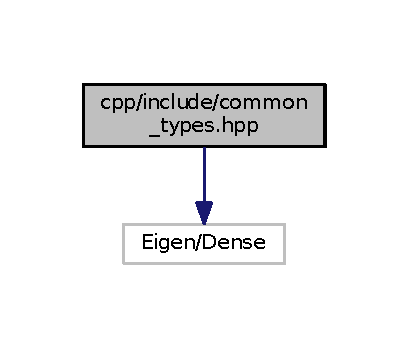
\includegraphics[width=196pt]{common__types_8hpp__incl}
\end{center}
\end{figure}
This graph shows which files directly or indirectly include this file\+:\nopagebreak
\begin{figure}[H]
\begin{center}
\leavevmode
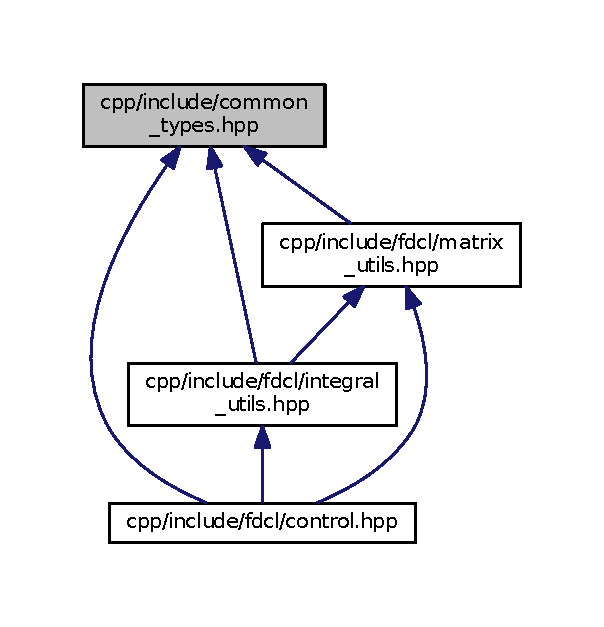
\includegraphics[width=290pt]{common__types_8hpp__dep__incl}
\end{center}
\end{figure}
\subsection*{Classes}
\begin{DoxyCompactItemize}
\item 
struct \hyperlink{structfdcl_1_1state__t}{fdcl\+::state\+\_\+t}
\begin{DoxyCompactList}\small\item\em Data structure to store current states. \end{DoxyCompactList}\item 
class \hyperlink{classfdcl_1_1command__t}{fdcl\+::command\+\_\+t}
\begin{DoxyCompactList}\small\item\em Data structure to store command (or desired) values. \end{DoxyCompactList}\end{DoxyCompactItemize}
\subsection*{Typedefs}
\begin{DoxyCompactItemize}
\item 
typedef Eigen\+::\+Matrix$<$ double, 2, 1 $>$ {\bfseries Vector2}\hypertarget{common__types_8hpp_adf06600ed595fddc4a8cab0f6cf96d61}{}\label{common__types_8hpp_adf06600ed595fddc4a8cab0f6cf96d61}

\item 
typedef Eigen\+::\+Matrix$<$ double, 3, 1 $>$ {\bfseries Vector3}\hypertarget{common__types_8hpp_a5db1d0e26b17aba6b7cc1ad4b18e248f}{}\label{common__types_8hpp_a5db1d0e26b17aba6b7cc1ad4b18e248f}

\item 
typedef Eigen\+::\+Matrix$<$ double, 4, 1 $>$ {\bfseries Vector4}\hypertarget{common__types_8hpp_a290681b9f47e358d1112b14eb952d6d8}{}\label{common__types_8hpp_a290681b9f47e358d1112b14eb952d6d8}

\item 
typedef Eigen\+::\+Matrix$<$ double, 3, 3 $>$ {\bfseries Matrix3}\hypertarget{common__types_8hpp_a550d61e84799433bdc546cc02655d4bc}{}\label{common__types_8hpp_a550d61e84799433bdc546cc02655d4bc}

\end{DoxyCompactItemize}


\subsection{Detailed Description}
Data types used throughout the code. 

Data structures and type definitions used are defined here. 
\hypertarget{control_8hpp}{}\section{cpp/include/fdcl/control.hpp File Reference}
\label{control_8hpp}\index{cpp/include/fdcl/control.\+hpp@{cpp/include/fdcl/control.\+hpp}}


Control class used to generate motors outputs for a desired trajectory.  


{\ttfamily \#include \char`\"{}common\+\_\+types.\+hpp\char`\"{}}\\*
{\ttfamily \#include \char`\"{}fdcl/param.\+hpp\char`\"{}}\\*
{\ttfamily \#include \char`\"{}fdcl/integral\+\_\+utils.\+hpp\char`\"{}}\\*
{\ttfamily \#include \char`\"{}fdcl/matrix\+\_\+utils.\+hpp\char`\"{}}\\*
{\ttfamily \#include \char`\"{}Eigen/\+Dense\char`\"{}}\\*
Include dependency graph for control.\+hpp\+:\nopagebreak
\begin{figure}[H]
\begin{center}
\leavevmode
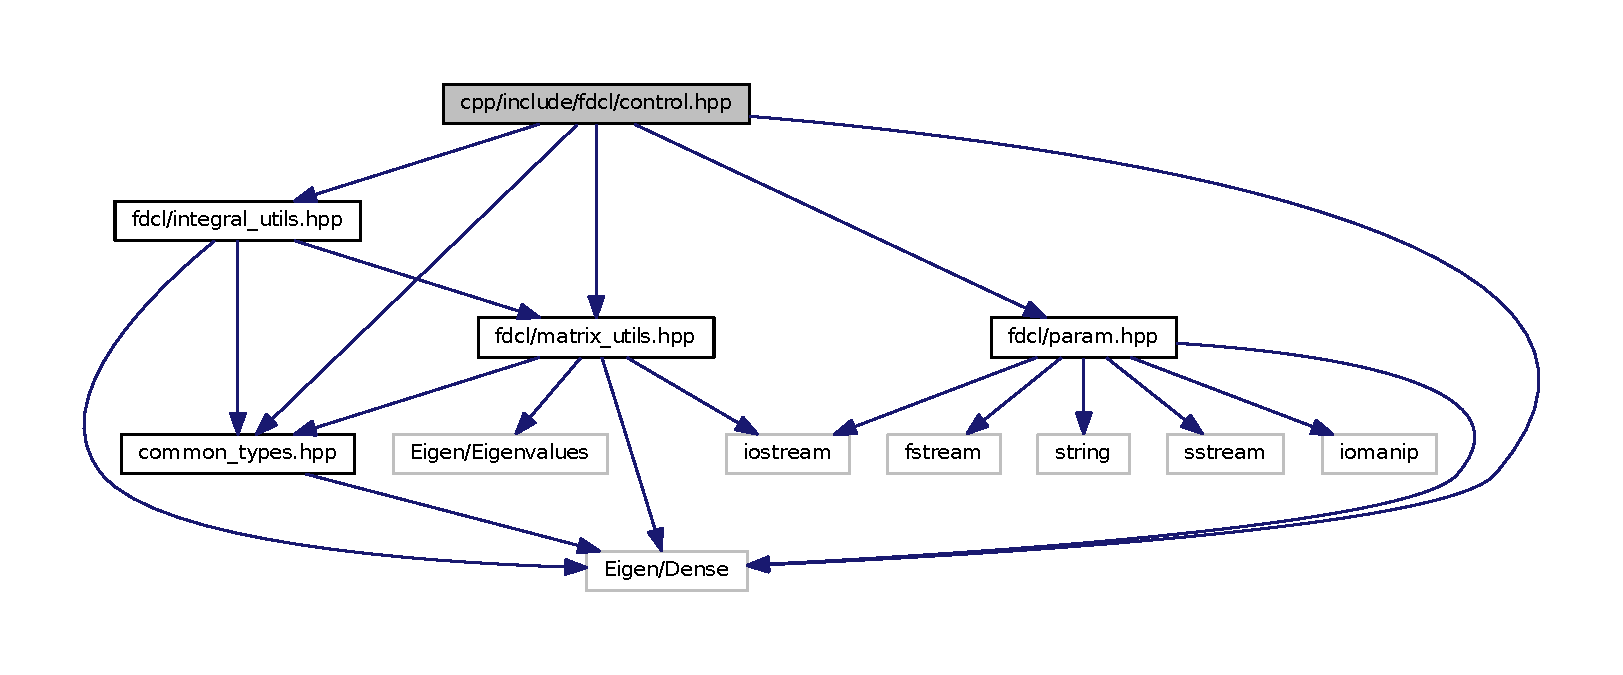
\includegraphics[width=350pt]{control_8hpp__incl}
\end{center}
\end{figure}
\subsection*{Classes}
\begin{DoxyCompactItemize}
\item 
class \hyperlink{classfdcl_1_1control}{fdcl\+::control}
\begin{DoxyCompactList}\small\item\em Controller functions for the rover. \end{DoxyCompactList}\end{DoxyCompactItemize}


\subsection{Detailed Description}
Control class used to generate motors outputs for a desired trajectory. 


\hypertarget{integral__utils_8hpp}{}\section{cpp/include/fdcl/integral\+\_\+utils.hpp File Reference}
\label{integral__utils_8hpp}\index{cpp/include/fdcl/integral\+\_\+utils.\+hpp@{cpp/include/fdcl/integral\+\_\+utils.\+hpp}}


Structures to handle integral errors.  


{\ttfamily \#include \char`\"{}common\+\_\+types.\+hpp\char`\"{}}\\*
{\ttfamily \#include \char`\"{}fdcl/matrix\+\_\+utils.\+hpp\char`\"{}}\\*
{\ttfamily \#include \char`\"{}Eigen/\+Dense\char`\"{}}\\*
Include dependency graph for integral\+\_\+utils.\+hpp\+:\nopagebreak
\begin{figure}[H]
\begin{center}
\leavevmode
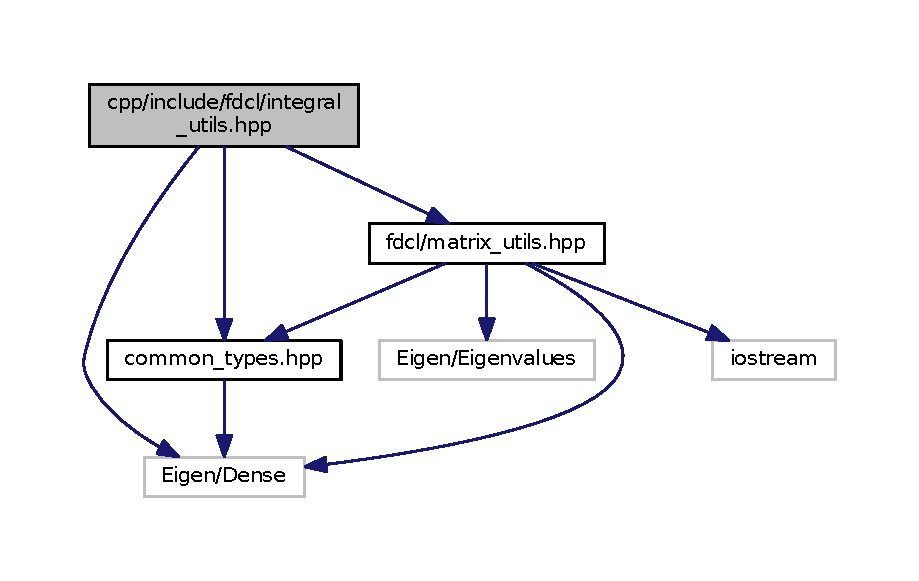
\includegraphics[width=350pt]{integral__utils_8hpp__incl}
\end{center}
\end{figure}
This graph shows which files directly or indirectly include this file\+:\nopagebreak
\begin{figure}[H]
\begin{center}
\leavevmode
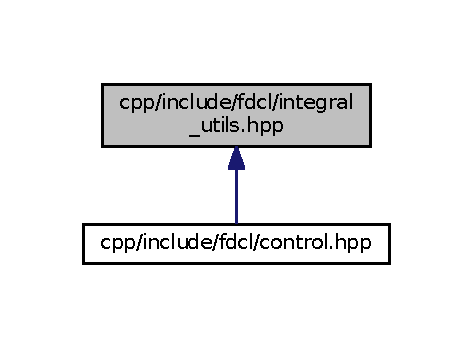
\includegraphics[width=227pt]{integral__utils_8hpp__dep__incl}
\end{center}
\end{figure}
\subsection*{Classes}
\begin{DoxyCompactItemize}
\item 
struct \hyperlink{structfdcl_1_1integral__error__vec3}{fdcl\+::integral\+\_\+error\+\_\+vec3}
\begin{DoxyCompactList}\small\item\em Integral for error for Vector3. \end{DoxyCompactList}\item 
struct \hyperlink{structfdcl_1_1integral__error}{fdcl\+::integral\+\_\+error}
\begin{DoxyCompactList}\small\item\em Integral for error for a double. \end{DoxyCompactList}\end{DoxyCompactItemize}


\subsection{Detailed Description}
Structures to handle integral errors. 


\hypertarget{matrix__utils_8hpp}{}\section{cpp/include/fdcl/matrix\+\_\+utils.hpp File Reference}
\label{matrix__utils_8hpp}\index{cpp/include/fdcl/matrix\+\_\+utils.\+hpp@{cpp/include/fdcl/matrix\+\_\+utils.\+hpp}}


Miscellaneous math functions.  


{\ttfamily \#include $<$iostream$>$}\\*
{\ttfamily \#include $<$Eigen/\+Dense$>$}\\*
{\ttfamily \#include $<$Eigen/\+Eigenvalues$>$}\\*
{\ttfamily \#include \char`\"{}common\+\_\+types.\+hpp\char`\"{}}\\*
Include dependency graph for matrix\+\_\+utils.\+hpp\+:\nopagebreak
\begin{figure}[H]
\begin{center}
\leavevmode
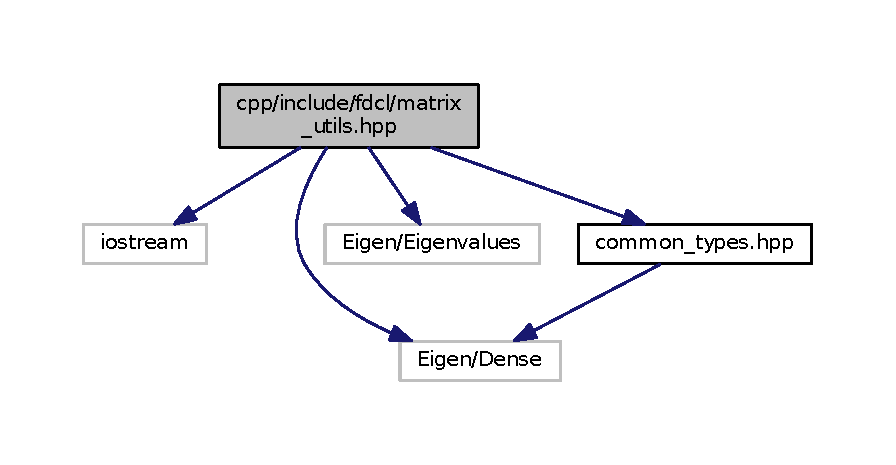
\includegraphics[width=350pt]{matrix__utils_8hpp__incl}
\end{center}
\end{figure}
This graph shows which files directly or indirectly include this file\+:\nopagebreak
\begin{figure}[H]
\begin{center}
\leavevmode
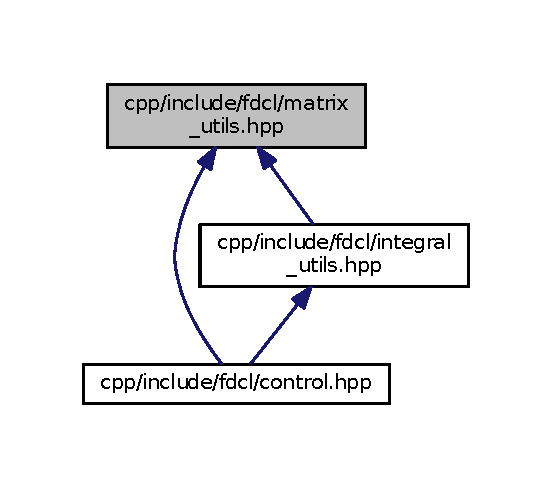
\includegraphics[width=265pt]{matrix__utils_8hpp__dep__incl}
\end{center}
\end{figure}
\subsection*{Functions}
\begin{DoxyCompactItemize}
\item 
Matrix3 \hyperlink{matrix__utils_8hpp_a09c674211aadc35e1a4af5800dd5637f}{hat} (const Vector3 v)
\item 
Vector3 \hyperlink{matrix__utils_8hpp_acc28574c8dae6766a23c4d26a6247e3d}{vee} (const Matrix3 V)
\item 
void \hyperlink{matrix__utils_8hpp_aecc1fdfb46dae124bcab57caaa3b4c85}{saturate} (Vector3 \&x, const double x\+\_\+min, const double x\+\_\+max)
\item 
void {\bfseries deriv\+\_\+unit\+\_\+vector} (const Vector3 \&A, const Vector3 \&A\+\_\+dot, const Vector3 \&A\+\_\+ddot, Vector3 \&q, Vector3 \&q\+\_\+dot, Vector3 \&q\+\_\+ddot)\hypertarget{matrix__utils_8hpp_aa1b124e027ab0c319b8ac6ef470003fd}{}\label{matrix__utils_8hpp_aa1b124e027ab0c319b8ac6ef470003fd}

\end{DoxyCompactItemize}


\subsection{Detailed Description}
Miscellaneous math functions. 

Miscellaneous math functions used in F\+D\+CL are defined here 

\subsection{Function Documentation}
\index{matrix\+\_\+utils.\+hpp@{matrix\+\_\+utils.\+hpp}!hat@{hat}}
\index{hat@{hat}!matrix\+\_\+utils.\+hpp@{matrix\+\_\+utils.\+hpp}}
\subsubsection[{\texorpdfstring{hat(const Vector3 v)}{hat(const Vector3 v)}}]{\setlength{\rightskip}{0pt plus 5cm}Matrix3 hat (
\begin{DoxyParamCaption}
\item[{const Vector3}]{v}
\end{DoxyParamCaption}
)}\hypertarget{matrix__utils_8hpp_a09c674211aadc35e1a4af5800dd5637f}{}\label{matrix__utils_8hpp_a09c674211aadc35e1a4af5800dd5637f}
Returns the hat map of a given 3x1 vector. This is the inverse of vee map. 
\begin{DoxyParams}{Parameters}
{\em v} & vector which the hat map is needed to be operated on \\
\hline
\end{DoxyParams}
\begin{DoxyReturn}{Returns}
hat map of the input vector 
\end{DoxyReturn}
\index{matrix\+\_\+utils.\+hpp@{matrix\+\_\+utils.\+hpp}!saturate@{saturate}}
\index{saturate@{saturate}!matrix\+\_\+utils.\+hpp@{matrix\+\_\+utils.\+hpp}}
\subsubsection[{\texorpdfstring{saturate(\+Vector3 \&x, const double x\+\_\+min, const double x\+\_\+max)}{saturate(Vector3 &x, const double x_min, const double x_max)}}]{\setlength{\rightskip}{0pt plus 5cm}void saturate (
\begin{DoxyParamCaption}
\item[{Vector3 \&}]{x, }
\item[{const double}]{x\+\_\+min, }
\item[{const double}]{x\+\_\+max}
\end{DoxyParamCaption}
)}\hypertarget{matrix__utils_8hpp_aecc1fdfb46dae124bcab57caaa3b4c85}{}\label{matrix__utils_8hpp_aecc1fdfb46dae124bcab57caaa3b4c85}
Saturate the elements of a given 3x1 vector between a minimum and a maximum value. 
\begin{DoxyParams}{Parameters}
{\em x} & vector which the elements needed to be saturated \\
\hline
{\em x\+\_\+min} & minimum value for each element \\
\hline
{\em x\+\_\+max} & maximum value for each element \\
\hline
\end{DoxyParams}
\index{matrix\+\_\+utils.\+hpp@{matrix\+\_\+utils.\+hpp}!vee@{vee}}
\index{vee@{vee}!matrix\+\_\+utils.\+hpp@{matrix\+\_\+utils.\+hpp}}
\subsubsection[{\texorpdfstring{vee(const Matrix3 V)}{vee(const Matrix3 V)}}]{\setlength{\rightskip}{0pt plus 5cm}Vector3 vee (
\begin{DoxyParamCaption}
\item[{const Matrix3}]{V}
\end{DoxyParamCaption}
)}\hypertarget{matrix__utils_8hpp_acc28574c8dae6766a23c4d26a6247e3d}{}\label{matrix__utils_8hpp_acc28574c8dae6766a23c4d26a6247e3d}
Returns the vee map of a given 3x3 matrix. This is the inverse of hat map. 
\begin{DoxyParams}{Parameters}
{\em V} & matrix which the vee map is needed to be operated on \\
\hline
\end{DoxyParams}
\begin{DoxyReturn}{Returns}
vee map of the input matrix 
\end{DoxyReturn}

%--- End generated contents ---

% Index
\backmatter
\newpage
\phantomsection
\clearemptydoublepage
\addcontentsline{toc}{chapter}{Index}
\printindex

\end{document}
